\begin{titlepage}

\begin{center}

% Oberer Teil der Titelseite:
%\includegraphics[width=0.15\textwidth]{./logo}\\[1cm]    
\textsc{\LARGE Produktentwicklung 2}\\[1.5cm]

\textsc{\Large Hochschule Luzern\\
    ~\\
    Technik \& Architektur}\\[0.5cm]

\vfill{}

% Title
\newcommand{\HRule}{\rule{\linewidth}{0.5mm}}
\HRule \\[0.4cm]
{   \Huge \bfseries Projektplanung\\
        ~\\
        \large Einführung in die Projektverwaltung mit GitHub}\\[0.4cm]

\HRule \\[1.5cm]

% Author and supervisor
\begin{minipage}{0.4\textwidth}
    \begin{flushleft} \large
        \emph{Autoren:}\\
        \textsc{Pren Team 39}\\
        Adriano \textsc{Valsangiacomo}\\
        Christian \textsc{Spycher}\\
        Christian \textsc{Schürch}\\
        Ervin \textsc{Mazlagi\'c}\\
        Fabian \textsc{Wüthrich}\\
        Alexander \textsc{Suter}\\
	Adrian \textsc{Würsch}
    \end{flushleft}
\end{minipage}
\hfill
\begin{minipage}{0.4\textwidth}
    \begin{flushright} \large
        \emph{Modulbetreuer:} \\
        Martin \textsc{Vogel}
    \end{flushright}
\end{minipage}

\vfill{}
\vfill{}
\vfill{}

% Unterer Teil der Seite
{\large Horw\\ \today}

\end{center}

\end{titlepage}
		% Titelseite
\thispagestyle{empty}

\begin{abstract}
Die erfolgreiche Realisierung eines Projektes verlangt nach einer
gewissen Struktur und Organisation. Diese liegen insbesondere im
Bereich der Planung und kontinuierlichen Kontrolle. Als Elementare
Intrumente gehören hierzu nach klassischen Modellen des
Projektmanagments die Meilensteine und Arbeitspakete.

In der vorligenden Arbeit soll zunächt eine kurze Einführung in die
theoretischen Aspekte dieser Instrumente gegeben werden. In einem 
weiteren Abschnitt wird die Methode des kollaborativen
Projemtmanagements soweit erläutert, wie es für die Verknüpfung für
die Verwendung mit GitHub notwendig ist. Die Beschreibung der
praktischen Umsetzung und der dazu eingesetzten Mittel stellt den
letzten Abschnitt der Arbeit dar, welcher auch einige Beispiele aus
der Umsetzung aufzeigt und Hinweise für die Verwendung gibt.
\end{abstract}
	% Abstract
\newpage
\tableofcontents		% Inhaltsverzeichnis
\newpage

%Beschreibung des Lösungskonzepts
\section{Management Summary}
Die vorliegende Dokumentation befasst sich mit der Umsetzung des Lösungskonzepts der Gruppe 39 für eine autonome Ballwurfmaschine.
Im Rahmen des Moduls PREN2 setzen wir uns mit dem Zusammenbau und dem Testen des Prototypen und dessen Funktionen auseinander.
Dazu wurden die Komponenten eingekauft und wenn notwendig angepasst. Von der Elektrotechnik wurden sämtliche Boards und Steuerungen bereitgestellt.
So kann die Informatik über bestimmte Schnittstellen optimal auf die Maschine zugreifen und diese steuern.
\newpage
\section{Einleitung}

Suchen, anvisieren und treffen. Zu Urzeiten waren diese Tätigkeiten überlebensnotwendig, wollte man etwas Fleisch zwischen die Zähne bekommen. Einige Zeitalter später steht man beinahe vor der gleichen Problemstellung. Jedoch soll kein Blut fliessen. Denn das Ziel ist kein lebendiges Tier sondern ein schwarzer, feststehender Korb. Dieser Korb muss gefunden werden, die Ausrichtung muss diesen anvisieren und schlussendlich müssen fünf Tennisbälle hinein befördert werden.

In der Aufgabenstellung wurde eine Ballwurfmaschine gefordert, welche nach einem Startsignal, selbständig den Korb findet und die Bälle hinein befördert. Das PREN Team 39 hat in einer ersten Phase ein Konzept für eine solche Maschine erarbeitet. Es wurden verschiedene Lösungsansätze verfolgt und nach einem einheitlichen Raster bewertet. Die Idee mit der höchsten Punktzahl wurde im Detail ausgearbeitet um diese schlussendlich in der zweiten Phase umzusetzen. Angehende Maschinenbau-, Elektrotechnik- und Informatik-Ingenieure setzten sich zusammen um das Konzept optimal umzusetzen. Die Interdisziplinarität spielt eine grosse Rolle und ist ein wesentlicher Bestandteil des Projekts.

In der vorliegenden Arbeit wird zuerst grob auf das Lösungskonzept eingegangen. Anschliessend werden in den einzelnen Disziplinen die Komponenten beschrieben. Der mechanische Aufbau, die Verkabelung der Elektrotechnik sowie die Architektur der Software sind festgehalten. Informationen zum Projektmanagement wie die Organisation, die Planung, die Kosten und das Risikomanagement liegen nachfolgend vor. Detaillierte Informationen sind im Anhang vorhanden.



\newpage
\section{Lösungskonzept}

\subsection{Produktbeschreibung}
\subsection{Übersichtszeichnung}
Die Ballwurfmaschine funktioniert nach einem einfachen Konzept. Der Ball wird in eine Verengung geschoben und durch ein Drehrad nach vorne gedrückt. Dadurch wird er beschleunigt und zielgerichtet auf seine Flugbahn gelenkt.
\begin{figure}[h!]
	\centering
	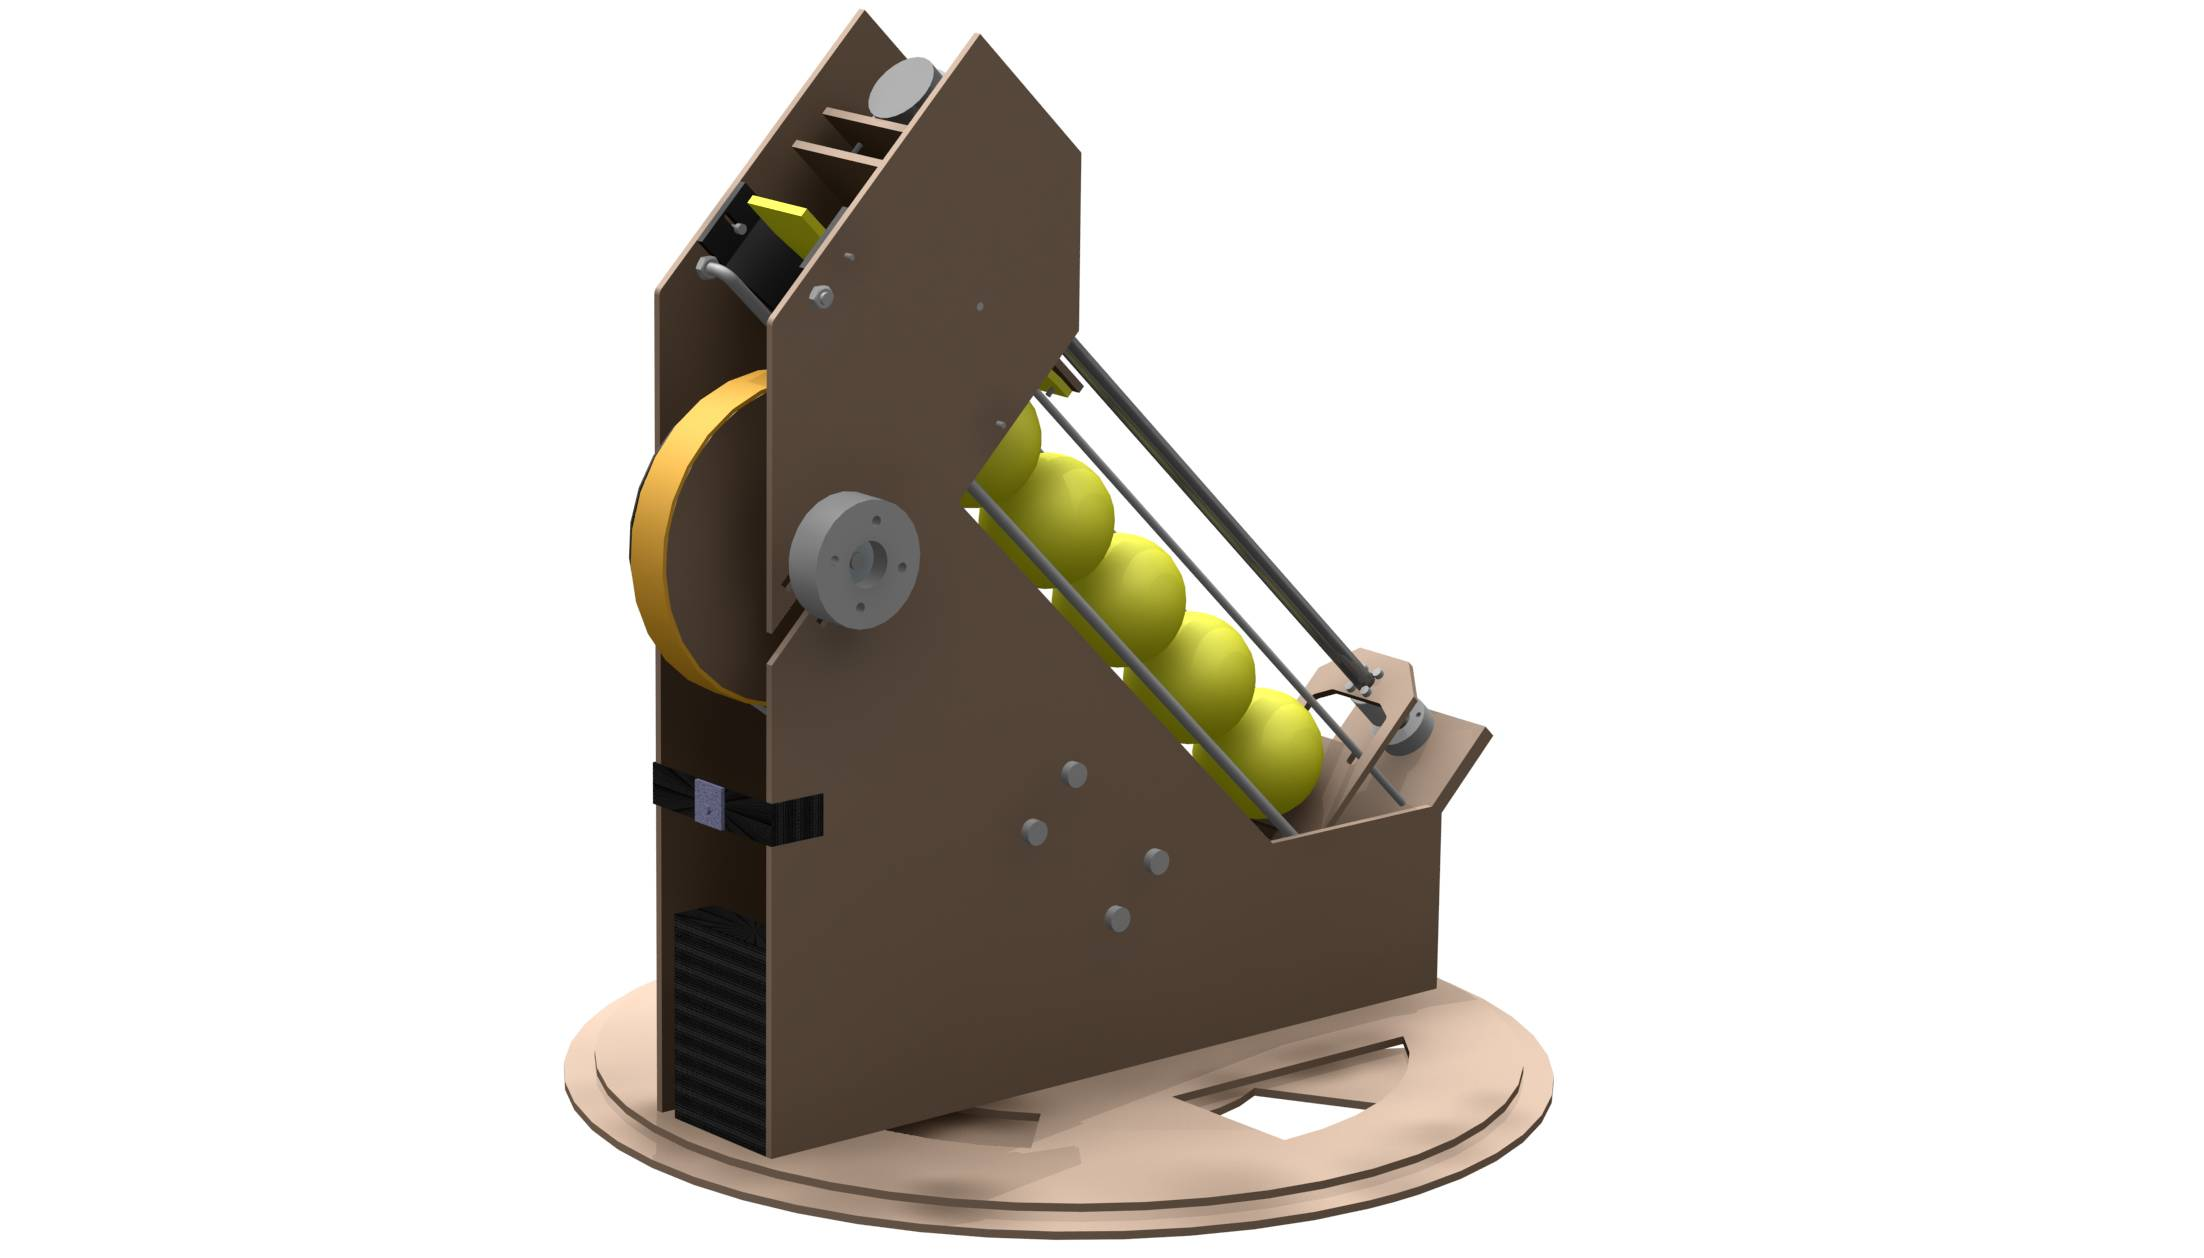
\includegraphics[width=\linewidth]{../../fig/Render_Komplettsystem}
	\caption{Übersichtszeichnung}
	\label{fig:Übersichtszeichnung}
\end{figure}
\newpage
\subsubsection{Blockdiagramm}
Das Blockdiagramm beschreibt den Zusammenhang der einzelnen Komponenten. In Abbildung \ref{fig:blockdiagramm} wird dies dargestellt. Die externe Steuerungseinheit (Notebook) greift über WLAN auf das Raspberry Pi zu. Dieses kommuniziert mit der PI-Kamera für die Detektion des Korbes. Zudem greift das Pi auf das Freedom Board zu, welches wiederum zuständig für alle Motoren ist. Die Turmausrichtung übernimmt der Stepper, die Beschleunigung des Schwungrades ist Sache des BLDC-Motors und für den Ballnachschub ist der DC-Motor zuständig.

\begin{figure}[h!]
\centering
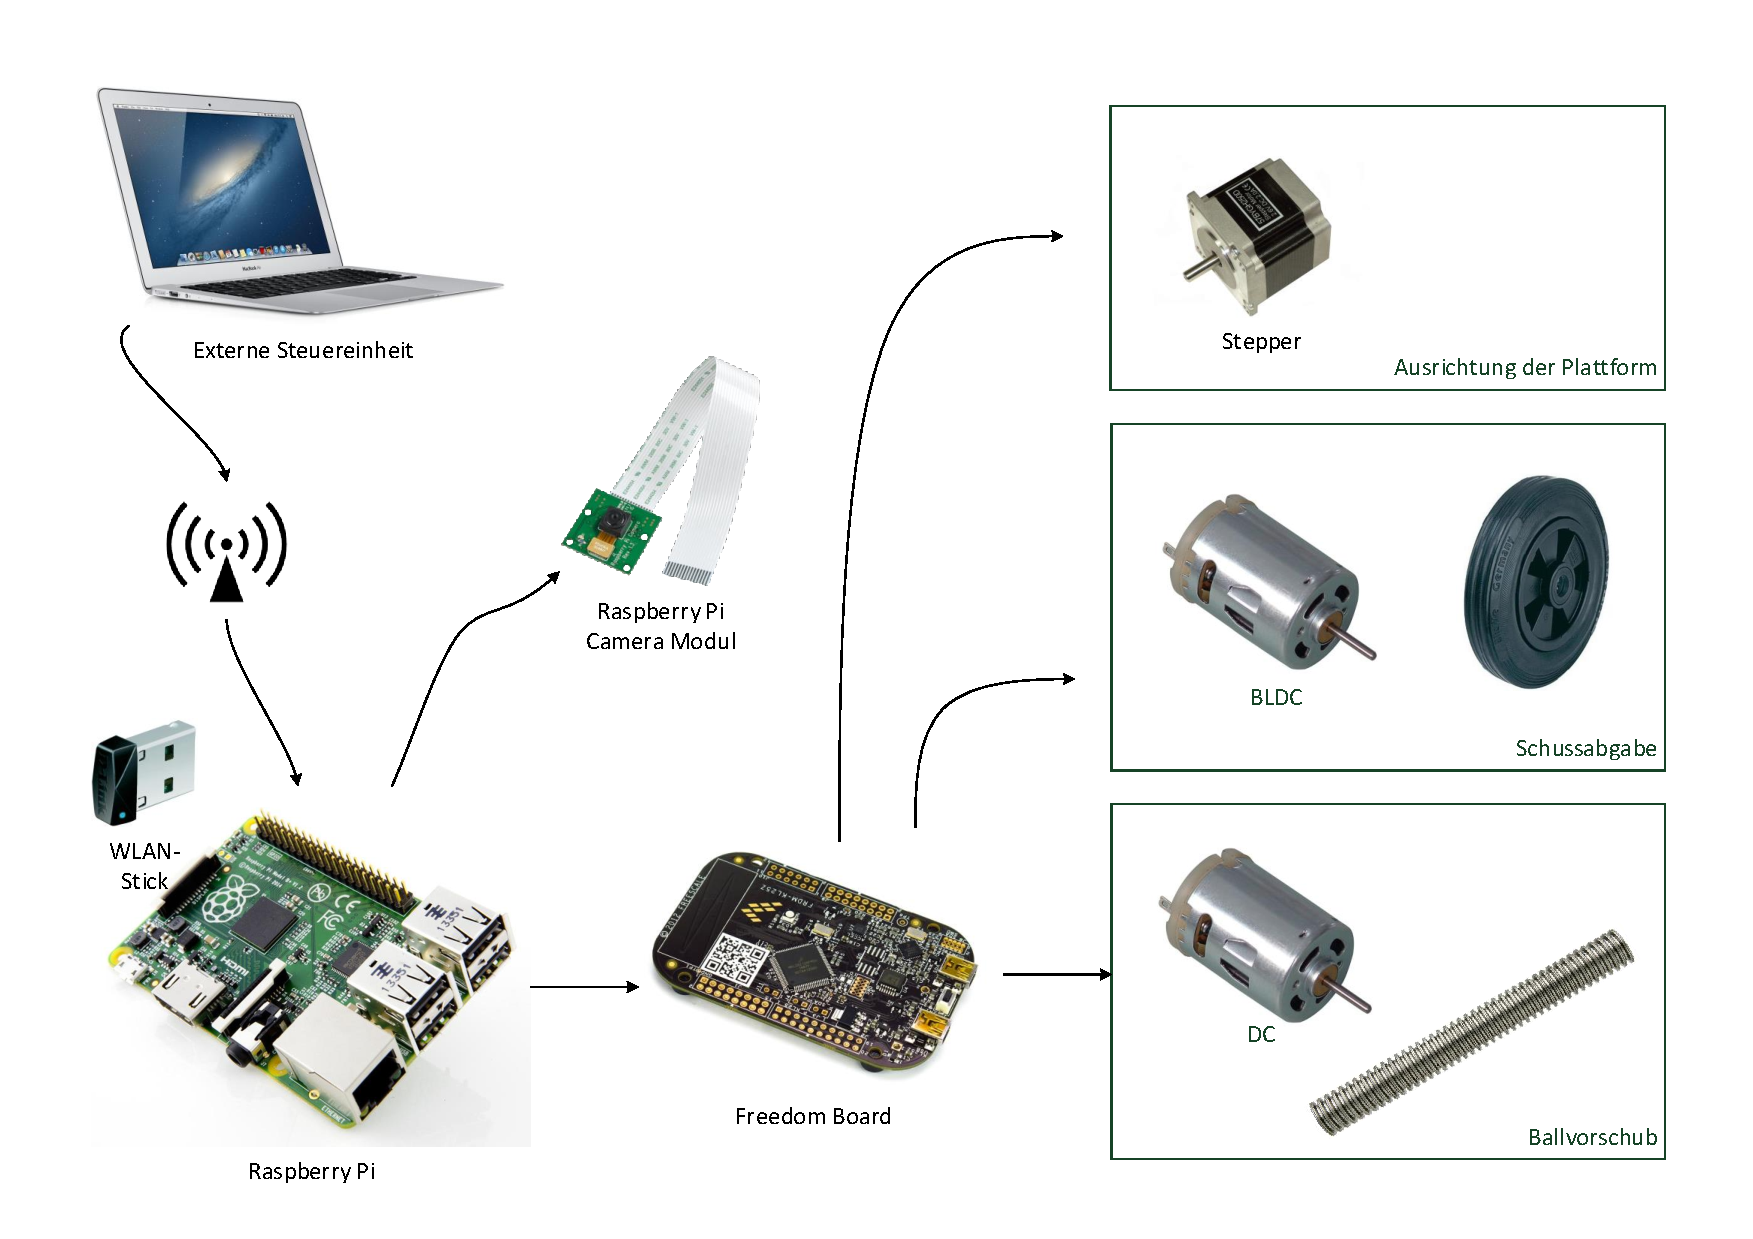
\includegraphics[width=0.9\linewidth]{../../fig/blockdiagramm}
\caption{Blockdiagramm}
\label{fig:blockdiagramm}
\end{figure}

\newpage
\subsubsection{Ablaufdiagramm}
Der allgemeine Ablauf der autonomen Wurfmaschine kann als endlicher Automat
modelliert werden, denn es gibt einen definierten Einstiegs- und 
Ausstiegspunkt. Der Einstieg (Start) ist definiert durch den Beginn der 5 minütigen Kalibrierung und der Ausstiegspunkt (Ende) ist gegeben, wenn der Ballvorschub den vorderen Endpunkt erreicht hat. Zwischen Start und Ende muss das Zielobjekt identifiziert, die Maschine ausgerichtet, die Wurfautomatik parametriert und schlussendlich der Wurf durchgeführt werden.

\begin{figure}[h!]
	\centering
	\begin{tikzpicture}[shorten >=2pt,node distance=4cm,on grid,auto]
	\node[state,initial] 	(q_0) 						{$q_0$};
	\node[state] 			(q_1) [above=of q_0]		{$q_1$};
	\node[state]			(q_2) [right=of q_1]		{$q_2$};
	\node[state]			(q_3) [right=of q_2]		{$q_3$};
	\node[state]			(q_4) [right=of q_3]		{$q_4$};
	\node[state,accepting]	(q_5) [below=of q_4]		{$q_5$};
	\path[->]
	(q_0)	edge node	{\begin{tabular}{c} Startsignal \end{tabular}} (q_1)
	(q_1)	edge node	{Korb entdeckt}	(q_2)
	(q_2)	edge node	{\begin{tabular}{c} Plattform \\ ausgerichtet \end{tabular}}	(q_3)
	(q_3)	edge node	{Drehzahl erreicht}	(q_4)
	(q_4)	edge node	{\begin{tabular}{c} Keine Bälle \\ vorhanden \end{tabular}}	(q_5);
	\end{tikzpicture}
	\caption{Autonome Wurfmaschine modelliert als endlicher Automat}
\end{figure}

\noindent
\textbf{Zustands- und Zustandsübergangsbeschreibungen}
\begin{itemize}
	
	\item Start \\ \\
	Gestartet wird nicht mit dem eigentlichen autonomen Prozess, sondern mit der Einrichtung der Maschine und der Kalibrierung.
	
	\item Kalibrierung ($q_{0}$) \\ \\
	Zu Beginn steht eine 5 minütige Kalibrierung zur Verfügung. In dieser Phase kann die Elektronik auf die Mechanik abgestimmt und allfällige Einstellungen am Bildverarbeitungssystem vorgenommen werden. Nach Ablauf dieser 5 Minuten darf keine Änderung am System mehr vorgenommen werden. Siehe dazu Anhang \ref{fig:ablauf-ballwurf}.
	
	\item Zustandsübergang von $q_{0}$ zu $q_{1}$ \\ \\
	Der eigentliche Prozess erfolgt nun mittels eines Start-Signales, welches von einer externen Steuerungseinheit drahtlos übermittelt wird.
	
	\item Ortung des Korbs ($q_{1}$) \\ \\
	Zur Ortung des Korbs wird ein Foto mit einer eingebauten Kamera gemacht. Dieses Foto wird mittels eines eigenen Algorithmus ausgewertet um den Ort zu bestimmen. Der Korb wird immer entdeckt, was jedoch nicht automatisch bedeutet, dass die richtige Position zurückgegeben wird. Denn statt das System stillzulegen, wenn der Korb nicht detektiert wird, kann man immer noch auf Basis des Zufalls erfolgreich sein.
	
	\newpage
	
	\item Zustandsübergang von $q_{1}$ zu $q_{2}$ \\ \\
	Sobald die Detektierung abgeschlossen ist, wird der einzustellende Winkel der Komponente, welche für die Ausrichtung zuständig ist, übermittelt.
	
	\item Plattform ausrichten ($q_{2}$) \\ \\
	Die Plattform wird anhand der Positionsdaten ausgerichtet.
	
	\item Zustandsübergang von $q_{2}$ zu $q_{3}$ \\ \\
	Sobald der Prozess zur Ausrichtung der Plattform vollzogen ist, wird in den nächsten Zustand gewechselt.
	
	\item Drehzahl erreichen ($q_{3}$) \\ \\
	Der Antrieb des Drehrades wird gestartet. Damit immer von den gleichen Anfangsbedingungen ausgegangen werden kann, muss zuerst eine vorher definierte Drehzahl erreicht werden. Es wird die Anlaufverzögerung des Motors abgewartet und gemessen ob die gewünschte Drehzahl erreicht wurde.
	
	\item Zustandsübergang von $q_{3}$ zu $q_{4}$ \\ \\
	Sobald die Soll-Drehzahl erreicht wurde, wird in den nächsten Zustand gewechselt. Die Drehzahl wird bis zum Ende des ganzen Abwurfs konstant bleiben. Es wird darauf verzichtet, das Rad nach jedem Wurf zu stoppen und wieder neu zu starten.
	
	\item Ballvorschub starten ($q_{4}$) \\ \\
	Die Ballwurfmaschine ist somit schussbereit. Als nächstes wird der Spindelantrieb des Ballvorschubes gestartet. Der Ballvorschub führt die Bälle an das Drehrad heran und die Bälle werden beschleunigt. 
	
	\item Zustandsübergang von $q_{4}$ zu $q_{5}$ \\ \\
	Sobald der Ballvorschub den vorderen Endpunkt erreicht hat, wurden alle Bälle abgeworfen und es kann in den nächsten Zustand gewechselt werden.
	
	\item Stoppsignal senden ($q_{5}$) \\ \\
	Die externe Steuerungseinheit, welche das Start-Signal abgegeben hat, erhält das Stoppsignal.
	
	\item Ende \\ \\
	Mit dem Erhalt des Stoppsignal ist der Prozess abgeschlossen.
	
\end{itemize}

\noindent
\textbf{Fehler-Szenarien}
Während des ganzen Ablaufs können Fehler auftreten. Fällt eine Teilfunktion aus, so soll nach Möglichkeit trotzdem immer in den nächsten Zustand gewechselt werden. Kann beispielsweise der Korb nicht detektiert werden, so soll ein Zufallswinkel dem nächsten Zustand übermittelt werden. Kann die Plattform nicht ausgerichtet werden, dann soll die Transition in den nächsten Zustand trotzdem erfolgen. Wird nicht die gewünschte Drehzahl erreicht, soll anschliessend trotzdem versucht werden die Bälle abzuschiessen. Das Motto bei einem Fehler ist somit immer Best-Effort. Es ist nicht nötig direkt in den $q_{5}$ zu wechseln. Jede Funktion kann trotzdem ausgeführt werden, wenn eine davor liegende Funktion nicht ausgeführt werden konnte.

\newpage
\newpage
\section{Schnittstellen}

\section{REST von Webserver}

Die Schnittstelle von der externen Steuereinheit zum Raspberry Pi wird über eine REST\footnote{Representational State Transfer}-Schnittstelle realisiert. Es wurden folgende Ressourcen definiert:
\begin{itemize}
	\item camera
	\item image
	\item start
\end{itemize}
Jede Ressource lässt sich mit HTML-Methoden (GET, PUT, POST usw.) abrufen oder verändern. Die Schnittstelle lässt sich ohne Authentifizierung nutzen und arbeiten mit dem JSON-Datenformat. Nachfolgend werden die einzelnen Ressourcen näher beschrieben.

\subsection{GET camera}

Diese Anfrage liefert die aktuellen Einstellungen der Bilderkennung zurück.

\subsubsection{Parameter}

\begin{tabular}{l p{16cm}}
	\textbf{config} & Die Konfiguration der Bilderkennung \\
	\textbf{roi} & Ist der Bereich in dem der Korb erkennbar ist (Region of Interest). Er ist definiert durch die Koordinaten der linken oberen Ecke (x,y) und einer Fläche (height, width). \\
	\textbf{contrast} & Ein Wert zwischen -100 und 100 für den Kontrast der Kamera. \\
	\textbf{greyscale} & \texttt{true} wenn ein Graustufen-Bild erzeugt werden soll. \\
	\textbf{quality} & Ein Wert zwischen 0 und 100 für die Qualität des JPEG-Bildes. \\
	\textbf{line} & Die Pixellinie welche analysiert werden soll um den Korb zu detektieren. \\
	\textbf{height} & Auf welcher Höhe soll die Pixellinie analysiert werden. Darf max. so hoch sein wie die ROI. \\
	\textbf{area} & Bei der Detektierung wird nicht nur eine Pixellinie untersucht. Mit \texttt{area} kann ein Band definiert werden in dem die Linien analysiert werden. \\
	\textbf{image} & Der URL zum Bild der Kamera. Bei jedem Aufruf wird ein neues Bild erstellt.
\end{tabular}

\subsubsection{Beispiel Request}

\texttt{GET} \\
\texttt{http://<raspberrypi-ip>/camera}

\subsubsection{Beispiel Result}

\begin{lstlisting}[caption=GET camera Result, label=lst:camera, tabsize=2]
{
	"config": {
		"roi": {
			"x": 100,
			"y": 200,
			"height": 300,
			"width": 400
		},
		"contrast": 50,
		"greyscale": true,
		"quality": 100,
		"line": {
			"height": 300,
			"area": 5
		}
	},
	"image": "http://<raspberrypi-ip>/image"
}
\end{lstlisting}

\subsection{PUT camera}

Diese Anfrage verändert die Einstellungen der Bilderkennung.

\subsubsection{Beispiel Request}

\texttt{PUT} \\
\texttt{http://<raspberrypi-ip>/camera} \\
Body siehe Listing \ref{lst:camera}

\subsubsection{Beispiel Result}

\begin{lstlisting}[caption=PUT camera Result, tabsize=2]
{
	"status": true
}
\end{lstlisting}

\subsection{GET image}

Diese Anfrage liefert das Bild der Kamera zurück. Bei jeder Anfrage wird ein Bild erstellt.

\subsubsection{Beispiel Request}

\texttt{GET} \\
\texttt{http://<raspberrypi-ip>/image}

\subsubsection{Beispiel Result}

Bild im JPEG-Format

\subsection{GET start}

Diese Anfrage liefert den Status des Vorgangs zurück. Wenn \texttt{start} auf \texttt{true} gesetzt ist läuft der Vorgang.

\subsubsection{Beispiel Request}

\texttt{GET} \\
\texttt{http://<raspberrypi-ip>/start}

\subsubsection{Beispiel Result}

\begin{lstlisting}[caption=GET start Result, tabsize=2]
{
	"start": true
}
\end{lstlisting}

\subsection{PUT start}

Diese Anfrage startet den Vorgang und übergibt die Callback-Adresse vom Steuergerät, damit der Stopp-Befehl zurück gesendet werden kann.

\subsubsection{Parameter}

\begin{tabular}{l p{16cm}}
	\textbf{start} & Bei \texttt{true} wird der Vorgang gestartet. Der Vorgang wird nicht unterbrochen falls \texttt{start} auf \texttt{false} gesetzt wird. Ist der Vorgang beendet wird \texttt{start} auf \texttt{false} gesetzt \\
	\textbf{url} & Die IP-Adresse des Steuergerätes. Diese wird benötigt um den Stopp-Befehl zurückzusenden.
\end{tabular}

\subsubsection{Beispiel Request}

\texttt{PUT} \\
\texttt{http://<raspberrypi-ip>/start}

\begin{lstlisting}[caption=PUT start Request, tabsize=2]
{
	"start": true,
	"url": "http://<steuergerät-ip>"
}
\end{lstlisting}

\subsubsection{Beispiel Result}

\begin{lstlisting}[caption=PUT start Result, tabsize=2]
{
	"status": true
}
\end{lstlisting}
\newpage
\subsection{Maschinenbau}
\subsubsection{Wurfmechanismus}
\subsubsection*{Komponentenbeschrieb}

Hauptstück des Wurfmechanismus ist das Wurfrad, welches durch Drehung um seine eigene Achse die Bälle beschleunigt.
Das aus fünf MDF-Tellern bestehende Wurfrad ist auf einer Aluminium-Achse montiert. Die Achse ist mit zwei an seinen Enden angebrachten Radiallagern mit den Seitenwänden des Drehturmes verbunden. Auf der Achse befindet sich ein Zahnriemenrad, welches über einen Zahnriemen die Verbindung zum antreibenden BLDC-Motor ermöglicht.
Um die Reibung zwischen den Bällen und dem Wurfrad zu erhöhen wurde ein Gummiband auf das Wurfrad geklebt.


\subsubsection*{Entwicklungsprozess}

Da der Wurfmechanismus die zentrale Einheit der Maschine darstellt, wurde ein spezielles Augenmerk auf ihn gerichtet. Würde er nicht funktionieren, wäre die gesamte Konstruktion untauglich. Nach diversen mehr oder weniger sinnvollen Lösungsansätzen, entschied man sich daher für eine der konservativeren Bauarten.
Das Wurfrad als beschleunigendes Element hat sich bei vielen anderen Tennisball-Wurfmaschinen bewährt und bot sich daher als sichere Lösung an.

\subsubsection{Ballnachschub}
\begin{figure}[h!]
	\centering
	\includegraphics[width=0.9\linewidth]{../../fig/Render-Ballnachschubx}
	\caption{Ballnachschub}
	\label{fig:Ballnachschub}
\end{figure}
\paragraph{Komponentenbeschrieb}
Der Ballnachschub wird mit einer rotierenden Trapezgewindespindel (TR10x3) und einem Mitnehmer sichergestellt. Die Tennisbälle werden seitlich mit Aluminiumstangen geführt und so in Richtung der Abwurfvorrichtung transportiert. Die Trapezgewindespindel ist auf der Unterseite mit einem Rillenkugellager gelagert. Auf der Oberseite wird die Lagerung mit einem Stehlager aus Kunststoff der Firma Igus realisiert. Ein DC-Motor treibt die Trapezgewindespindel an. Die Kraftübertragung vom DC-Motor auf die Trapezgewindespindel erfolgt mit zwei Kunststoff Stirnrädern. Das Übersetzungsverhältnis hierbei beträgt 2.67.

\paragraph{Entwicklungsprozess}
In einem ersten Entwurf wurde die Trapezgewindespindel auf der Unterseite auch mit einer Gleitführung realisiert. Dies funktionierte für den Ballnachschub einwandfrei. Wurde nach dem Ballabwurf die Drehrichtung umgekehrt, um den Mitnehmer zurück in die Startposition zu bringen, ergaben sich jedoch einige Probleme. Wegen der realisierten Gleitführung konnte sich die Trapezgewindespindel in axialer Richtung frei bewegen. Dadurch wurde die Spindel beim Zurückstellen tendenziell nach oben gezogen. Dies führte zu hörbaren Schwingungen, welche ein automatisches Zurückfahren erschwerten. Mit der angepassten Lagerung tritt dieses Problem nicht mehr auf. 
Eine weitere Knacknuss war die Führung der Bälle und dadurch das Finden der optimalen Position für die Führungsstangen. Da Tennisbälle eine runde Form besitzen, neigen sie dazu sich gegenseitig wegzudrücken. Daher mussten wir vier Aluminiumstangen als Führung verwenden. In einer ersten Version waren nur zwei Stangen auf der Unterseite vorgesehen. 
Beim ersten Entwurf endeten alle Führungsstangen auf der Höhe des Drehrades. Dies führte dazu, dass die Tennisbälle nach dem Abwurf, die Maschine auf einer horizontalen Flugbahn verliessen und nicht wie vorgesehen unter einem Winkel von 45° zur horizontalen Ebene. Dieses Problem konnte durch einer Verlängerung der Führungsstangen bis nach dem Drehrad verhindert werden. 
Der DC Motor wird mit einer Rohrschelle befestigt. Dabei wurde die Platte, auf welcher die Rohrschelle befestigt ist, im richtigen Abstand positioniert, so dass die Übersetzung realisiert werden kann. Dies stellt keine optimale Lösung dar. Da die Funktion jedoch erfüllt ist, wird auf eine Verbesserung verzichtet. 


\subsubsection{Ausrichtung Drehturm}
\begin{figure}[h!]
	\centering
		\includegraphics[width=\linewidth]{../../fig/Render-Drehmechanismusx}
	\caption{Drehmechanismus}
	\label{fig:Drehmechanismus}
\end{figure}
\paragraph{Komponentenbeschrieb\\}
Die horizontale Ausrichtung der Maschine in Richtung des Korbes, wird mittels einem Schrittmotor ermöglicht. An der Antriebswelle des Motors ist ein Kunststoff-Zahnrad angebracht, welches in ein eigens konstruiertes Hohlrad-Segment eingreift und somit durch Rotation eine Drehung des Drehturmes bewirkt. Dieses Segment ist auf der Grundplatte befestigt, welche fix auf dem Tisch liegt. Die zwei Platten, sowie das Hohlrad-Segment wurden mit NX konstruiert und mit einer Laserschneidmaschine aus MDF gefertigt.

\paragraph{Entwicklungsprozess\\}
Gemäss Aufgabenstellung sollen sich nach Abschluss des Wurfvorganges fünf Bälle im Korb befinden. Da die Position des Korbes nicht fix vorgegeben ist, können die Bälle nicht einfach nach vorne befördert werden. Um die Wurfvorrichtung ausrichten zu können, musste daher ein weiterer Aktor her. Grundsätzlich standen zwei Lösungskonzepte zur Auswahl. Ein seitliches Verschieben der kompletten Maschine, oder eine stationäre Variante mit einem Drehturm. Da eine seitliche Verschiebung in vielerlei Hinsicht schwieriger auszuführen wäre, entschied man sich für die Eigenrotation. Aus Montage- und Kostengründen verzichtete man bei der Lagerung zwischen den beiden Grundplatten auf ein genormtes Lager, obwohl dieses in der Planung vom PREN 1 vorgesehen wurde. Dieses Lösungskonzept verursacht jedoch eine höhere Reibung, weshalb der Schrittmotor eine grössere Leistung aufweisen muss. Dies stellt für den gewählten Motor allerdings kein Problem dar.

\subsubsection{Drehturm}
\begin{figure}[h!]
	\centering
	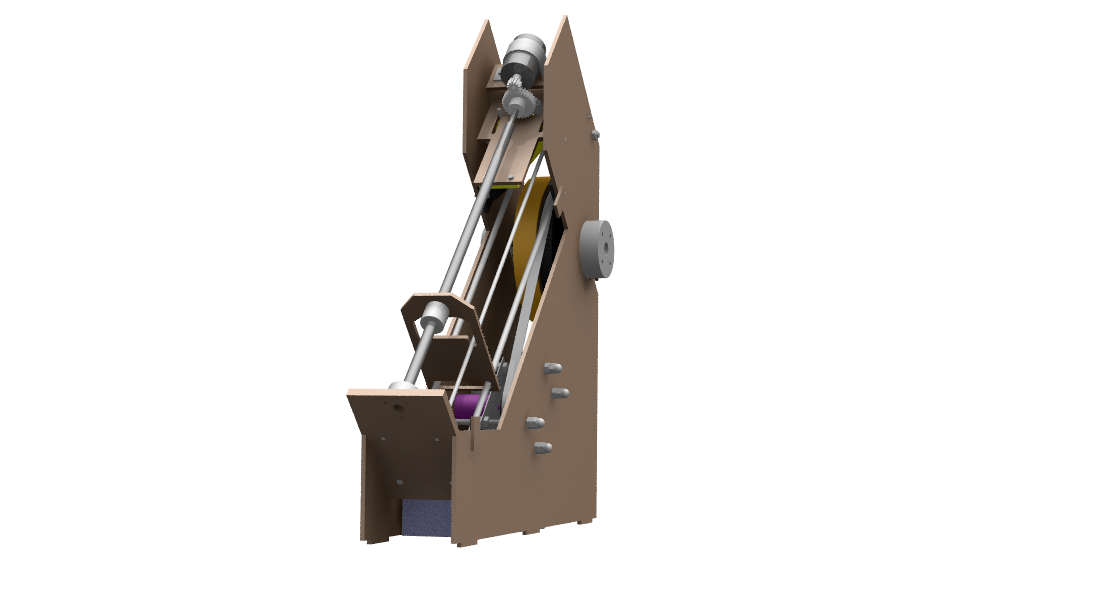
\includegraphics[width=\linewidth]{../../fig/Drehturm}
	\caption{Drehturm}
	\label{fig:Drehturm}
\end{figure}

\paragraph{Komponentenbeschrieb\\}
Der Drehturm ist das Gerüst, welches die verschiedenen Komponenten in den gewünschten Positionen hält. Er besteht aus zwei durch einen Laser zugeschnittenen MDF-Platten (Mitteldichte Holzfaserplatte) und ist durch Steckverbindungen auf dem Drehteller befestigt. Die Platten stehen parallel in einem Abstand von acht Zentimetern zueinander und umgeben somit die meisten Komponenten der Wurfmaschine. Die Vorrichtung wirkt durch diese Bauart auch ohne komplizierte Massnahmen aufgeräumt.

\paragraph{Entwicklungsprozess\\}
Schon während der frühen Entwicklungsphase des Konzeptes einigte man sich darauf, hauptsächlich durch Laserschneiden herstellbare Einzelkomponenten zu verwenden. Die Auswahl des Grundmaterials wurde daher eingeschränkt, da beispielsweise Metalle auf den Laseranlagen der Schule nur schlecht, bis gar nicht zu fertigen sind. Die Entscheidung fiel auf MDF, da dieser Werkstoff auch nach dem Laserschneiden noch gut zu bearbeiten ist. Die Form des Turmes ergab sich mehr oder weniger durch die Auswahl der Komponenten. Da ein linearer Ballnachschub gewählt wurde und die Platzverhältnisse begrenzt sind, musste in die Höhe konstruiert werden.

\subsubsection{Anpressvorrichtung}

\paragraph{Komponentenbeschrieb}
Damit mit verschiedenen Tennisballdurchmessern zuverlässig geschossen werden kann, ist die Anpressvorrichtung mit einer Federkonstruktion ausgestattet. Der Anpressdruck der Tennisbälle auf das Drehrad wird so konstant gehalten. Da die gewählte Bauform sensibel auf Änderungen des Anpressdruckes reagiert, musste dieser Komponente besondere Beachtung geschenkt werden. 

\paragraph{Entwicklungsprozess}
Die Anpressvorrichtung wurde während dem PREN 2 einige Male umkonstruiert und angepasst. In einem ersten Entwurf war die Position des Abwurfes falsch gewählt. Dies führte dazu, dass die Tennisbälle die Maschine nicht wie gewünscht verliessen. Ein anpressen der Bälle an das Drehrad mit einem elastischen Kunststoff wurde zudem als genügend gut erachtet. Da sich dies in der Ausführung allerdings als nicht zufriedenstellend herausstellte, wurde eine Konstruktion mit Federn erstellt. Um eine funktionierende Befestigung für die Federn zu finden, wurden ebenfalls einige Konstruktionen realisiert. Bei zu geringem Anpressdruck ist die Wurfdistanz zu gering. Analog dazu ist sie zu gross bei zu starkem Anpressdruck. Eine Schwäche zeigt sich jedoch auch bei der gefederten Konstruktion. Da die Federkraft und dadurch auch der Anpressdruck mit steigendem Federweg zunehmen, kann die Wurfdistanz nach wie vor variieren. Dies passend auszulegen war recht zeitintensiv.

\subsubsection{Komplettsystem}

\paragraph{Komponentenbeschrieb}

\paragraph{Entwicklungsprozess}

\newpage
\subsection{Informatik}

\subsubsection{Architektur}

Die Architektur lässt sich grob in zwei Komponenten (Fotoshoot UI/Raspi Controller) einteilen. Das Komponentendiagramm in Abbildung \ref{fig:komponentendiagramm} zeigt eine Übersicht über die Architektur. Beim Fotoshoot UI handelt es sich um ein Java Programm welches auf einem beliebigen Computer mit Java ausführen lässt. Es dient zur Steuerung der Maschine. Der Raspi Controller wird auf dem Raspberry Pi ausgeführt und verarbeitet die Befehle vom Fotoshoot UI.

\begin{figure}
	\centering
	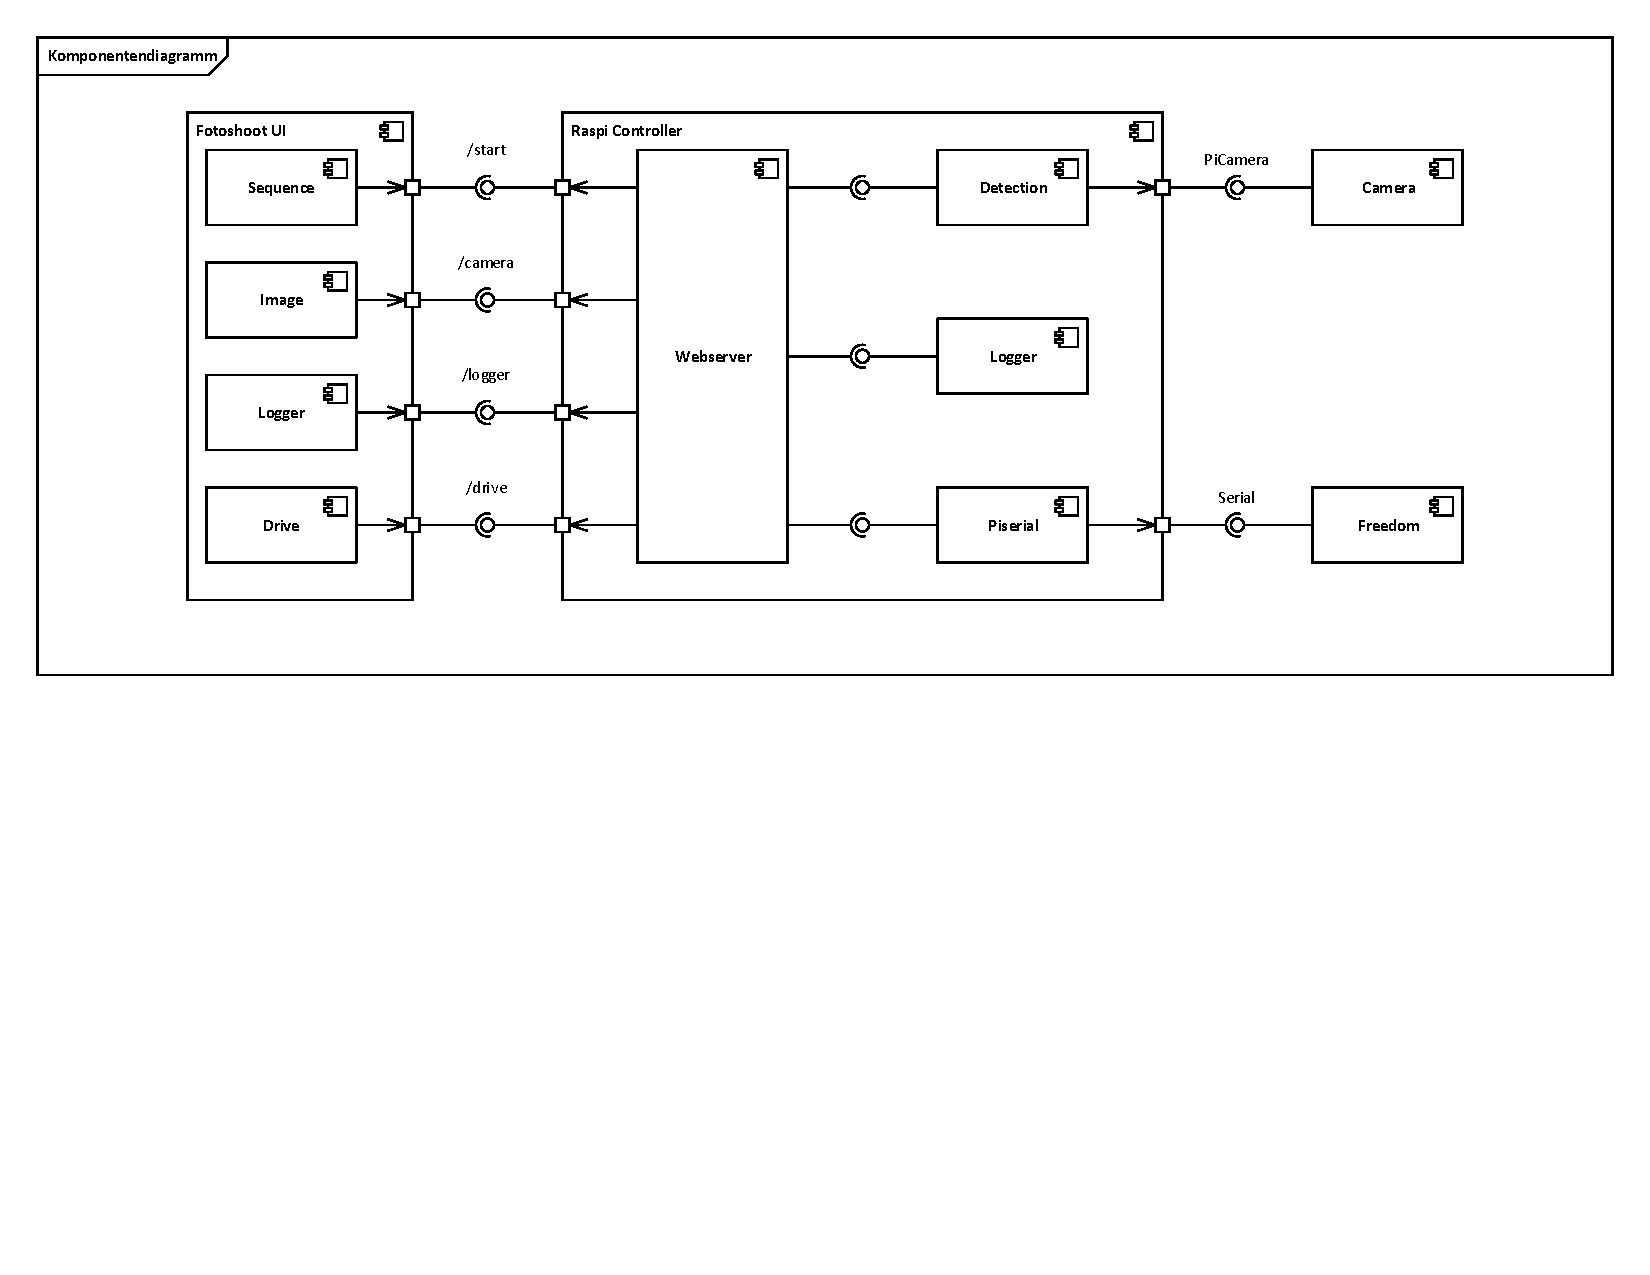
\includegraphics[width=\linewidth]{../../fig/komponentendiagramm}
	\caption{Komponentendiagramm}
	\label{fig:komponentendiagramm}
\end{figure}

Auf dem Raspi Controller wird ein Webserver ausgeführt, welcher über eine REST-Schnittstelle Befehle entgegen nimmt. Diese REST-Schnittstelle ermöglicht eine unabhängige Entwicklung der beiden Komponenten. Die Anfragen an der Webserver werden an weitere Komponenten innerhalb des Raspi Controllers weitergeleitet. Die Komponenten vom Raspi Controller wurde gemäss den Hauptfunktionen der Maschine aufgeteilt. Die Detection-Komponente erzeugt mit Hilfe der Camera-Komponente ein Bild und erkennt darauf den Korb. Die PiSerial-Komponente ist für die Ansteuerung der seriellen Schnittstelle und damit für die Kommunikation mit dem Freedom-Board zuständig. Mit dem Freedom-Board werden sämtliche Motoren angesteuert. Zusätzliche wurde noch eine Logger-Komponente entwickelt, welche für das Logging zuständig ist. Die Log-Einträge können über den Webserver abgerufen und auf dem UI dargestellt werden.

Die Komponenten vom Fotoshoot UI wurden gemäss den UI-Ansichten aufgeteilt. So gibt es beispielsweise eine UI-Ansicht für die Steuerung der Motoren. Alle Funktionen welche für diese Aufgabe benötigt werden, sind demzufolge in der Drive-Komponente zu finden.
\newpage
\subsubsection{Fotoshoot UI}

Das Fotoshoot UI hat mehrere Funktionen. Es dient um den Ballwurf-Prozess zu starten, die Korberkennung zu kalibrieren und die Motoren anzusteuern.

\paragraph{Starten des Ballwurfs (Komponente Sequence)}
Der gesamte Prozess kann mittels Start-Knopf gestartet werden. Die Benutzeroberfläche wird eingefroren und die Stoppuhr gestartet. Sobald der Prozess beendet wurde, wird die vergangene Zeit angezeigt.

\begin{figure}[h!]
\centering
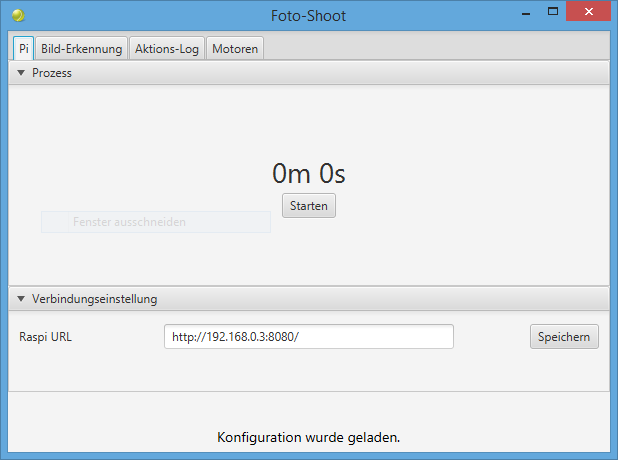
\includegraphics[width=0.6\linewidth]{../../fig/fotoshoot-ui/fotoshoot-ui-pi}
\caption{Fotoshoot-UI Prozess starten}
\label{fig:fotoshoot-ui-pi}
\end{figure}

\paragraph{Kalibrierung der Bildverarbeitung (Komponente Image)}
In diesem Bereich können die Parameter für die Bild-Erkennung definiert werden. Die Bedeutung der Parameter sowie die gültigen Werte sind in der Tabelle \ref{tab:parameter-bilderkennung} detailliert beschrieben. Im unteren Abschnitt dieses Tabs kann das Bild angezeigt werden. Auf dem Bild ist der erkannte Korb mit einem Fadenkreuz markiert.

\begin{figure}[h!]
	\centering
	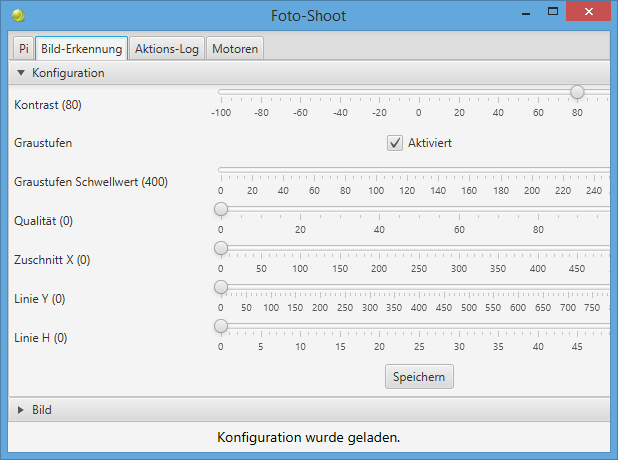
\includegraphics[width=0.6\linewidth]{../../fig/fotoshoot-ui/fotoshoot-ui-korb-erkennung}
	\caption{Fotoshoot-UI Bilderkennung}
	\label{fig:fotoshoot-ui-korb-erkennung}
\end{figure}

\paragraph{Ansteuerung der Motoren (Komponente Drive)}
Die einzelnen Motoren können über die Benutzeroberfläche angesteuert werden. Dies vereinfacht das Testen der einzelnen Komponenten massiv und macht es auch für alle zugänglich. Es braucht nun kein spezielles IT-Know-How mehr um die einzelnen Komponenten zu starten.

\begin{figure}[h!]
	\centering
	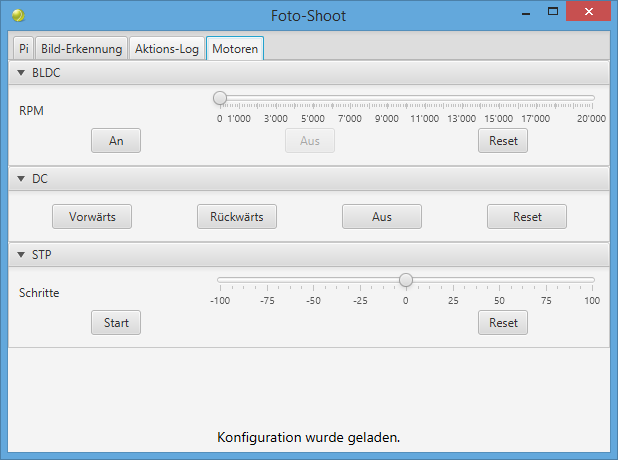
\includegraphics[width=0.6\linewidth]{../../fig/fotoshoot-ui/fotoshoot-ui-motoren}
	\caption{Fotoshoot-UI Ansteuerung der Motoren}
	\label{fig:fotoshoot-ui-motoren}
\end{figure}

\paragraph{Log (Komponente Logger)}
Während des Ballwurfs werden Log-Einträge erstellt. Die Logger-Komponente kann diese abfragen und bringt diese auf dem Tab Log zur Darstellung.

\begin{figure}[h!]
	\centering
	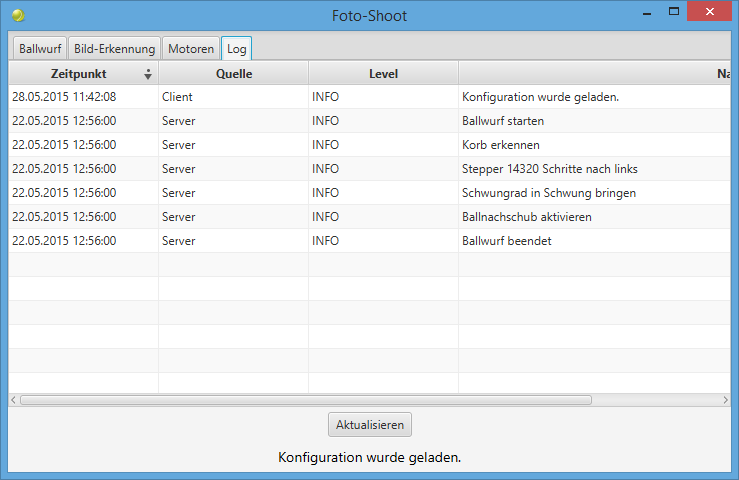
\includegraphics[width=0.6\linewidth]{../../fig/fotoshoot-ui/fotoshoot-ui-log}
	\caption{Fotoshoot-UI Log Einträge}
	\label{fig:fotoshoot-ui-log}
\end{figure}

\newpage

\paragraph{Technische Umsetzung}
Das Fotoshoot-UI wurde in Java und mit der heute aktuellen UI-Technologie Java-FX implementiert. Zudem sind zentral zwei 3rd-Parties Bibliotheken, welches den Bau dieser Applikation massiv vereinfachen soll.

\begin{description}
	\item[Google Guice:] Dies ist ein Depedency Injection Framework. Die Controller können nun ihre zusätzlichen Abhängigkeiten über die Injektion erhalten. Der Objekt-Baum muss nicht mehr mühsam von Hand erzeugt werden.
	\item[Eventbus:] Der Eventbus ist Teil von Google Guava. Dieser vereinfacht die Implementation des Observer-Patterns. Jeder kann auf den Eventbus Events senden und sich mit lediglich der Annotation \texttt{@Subscribe} für Events registrieren.
\end{description}
\begin{figure}[h!]
	\centering
	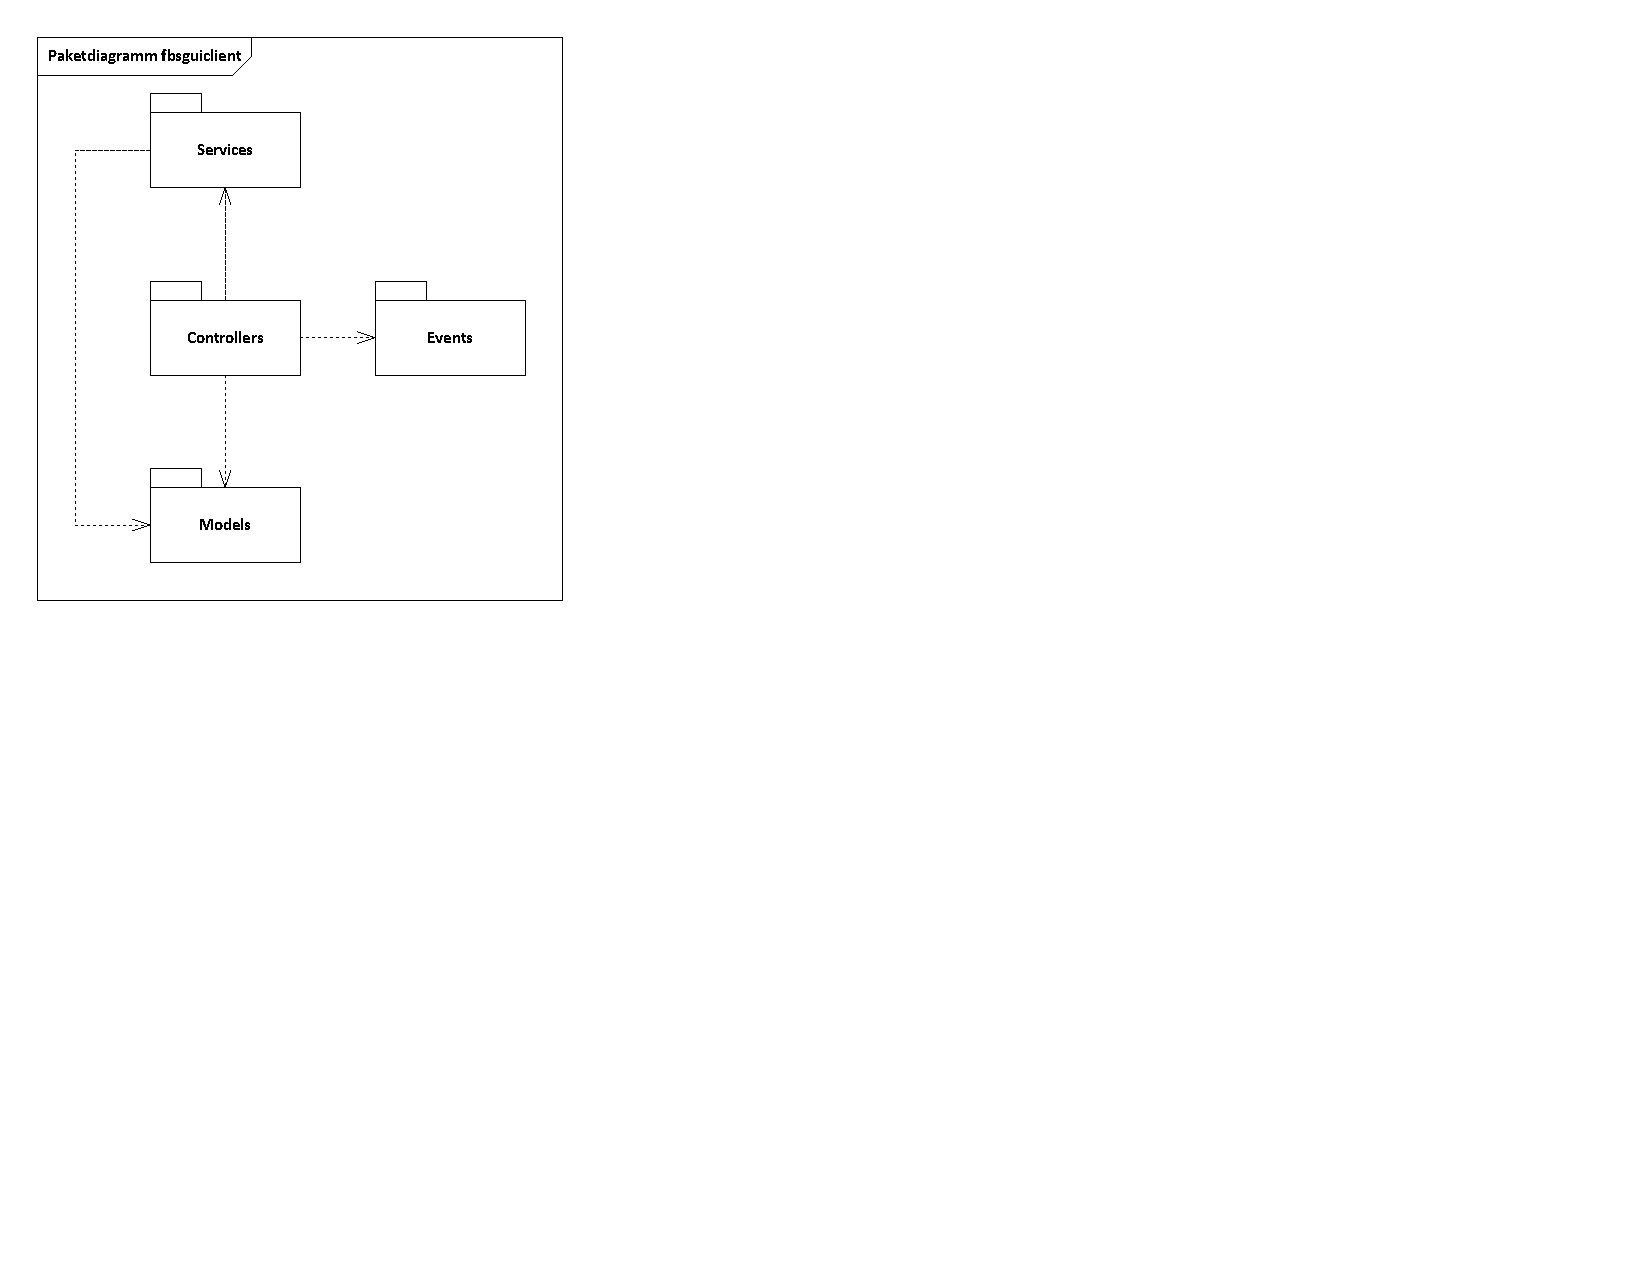
\includegraphics[width=0.4\linewidth]{../../fig/fotoshoot-ui/fotoshoot-ui-paketdiagramm}
	\caption{Paketdiagramm Fotoshoot-UI}
	\label{fig:fotoshoot-ui-paketdiagramm}
\end{figure}
Auf der Abbildung \ref{fig:fotoshoot-ui-paketdiagramm} ist zu erkennen wie die Applikation aufgebaut ist. Nachfolgend werden die einzelnen Pakete erklärt:
		
\begin{description}
	\item[Controller:] Die Controller beinhalten die FXML-Dateien und die konkreten Controller Klassen. Sie sind für die Benutzer-Aktionen, Service-Calls, sowie die Beziehung zwischen Modell und UI zuständig.
	\item[Modell:] Dies sind die Modelle fürs GUI. Diese sind fürs GUI zugeschnitten. Die Modelle beinhalten die Properties, welche über die Controller in die Views gebunden werden.
	\item[Services:] Diese sind zuständig für die Daten. Sowohl Daten-Abfrage und auch Manipulation. Sie stellen die Schnittstelle zum Business-Layer dar.
	\item[Events:] Das sind POJOs, welche von den Controller verwendet werden. Diese werden für die Kommunikation der Controller untereinander über den Eventbus benötigt.
\end{description}
Jeder Controller kann der Ursprung für eine Benutzeraktion sein, welcher Einfluss auf irgendwelche Views hat. Diesen Views liegen auch Controller zugrunde. Damit nicht jeder Controller jeden anderen Controller kennen muss, verwenden wir hier den Eventbus von Google. Jeder Controller wird automatisch registriert und kann über den Eventbus Events senden und sich für jedes Event auch wieder registrieren.

\newpage
\subsubsection{Raspi-Controller}
\newpage
\subsubsection{REST Schnittstelle}
\label{sec:rest-schnittstelle}

Die Schnittstelle von der externen Steuereinheit zum Raspberry Pi wird über eine REST\footnote{Representational State Transfer}-Schnittstelle realisiert. Es wurden folgende Ressourcen definiert:
\begin{itemize}
	\item \texttt{start}
	\item \texttt{camera}
	\item \texttt{drive}
	\item \texttt{logger}
\end{itemize}
Jede Ressource lässt sich mit HTTP-Methoden (\texttt{GET}, \texttt{PUT}, \texttt{POST} usw.) abrufen oder verändern. Die Schnittstelle lässt sich ohne Authentifizierung nutzen und arbeiten mit dem JSON-Datenformat. Nachfolgend werden die einzelnen Ressourcen näher beschrieben.

\paragraph{\texttt{GET /camera}}

Diese Anfrage liefert die aktuellen Einstellungen der Bilderkennung zurück. Nachfolgenden sind die Parameter der Kamera dokumentiert.
\label{tab:parameter-bilderkennung}
\begin{table}[h!]
	\begin{tabular}{l p{16cm}}
		\texttt{config} & Die Konfiguration der Bilderkennung \\
		\texttt{line\_y} & Die Pixellinie welche analysiert werden soll um den Korb zu detektieren. \\
		\texttt{line\_h} & Bei der Detektierung wird nicht nur eine Pixellinie untersucht. Mit \texttt{area} kann ein Band definiert werden in dem die Linien analysiert werden. \\
		\texttt{greyscale\_threshold} & Schwellenwert der Objekterkennung. \\
		\texttt{greyscale} & \texttt{true} wenn ein Graustufen-Bild erzeugt werden soll. \\
		\texttt{quality} & Ein Wert zwischen 0 und 100 für die Qualität des JPEG-Bildes. \\
		\texttt{crop\_x} & Breite des Feldes das auf beiden Seiten des Bildes abgeschnitten wird. \\
		\texttt{contrast} & Ein Wert zwischen -100 und 100 für den Kontrast der Kamera. \\
	\end{tabular}
	
\end{table}

\begin{table}[h!]
	\centering
	\begin{tabular}{|l|l|}
		\hline Anfrage an Raspberry Pi & Antwort von Raspberry Pi \\ 
		\hline \texttt{GET /camera HTTP/1.1} & \texttt{200 OK} \\
		\texttt{Host: <raspberrypi-ip>} & \texttt{Content-Type: text/json} \\
		& \\
		& \verb|{| \\
		& \verb|"greyscaleThreshold": 9,| \\
		& \verb|"cropX": 295,| \\
		& \verb|"lineY": 800,| \\
		& \verb|"lineH": 1,| \\
		& \verb|"greyscale": false,| \\
		& \verb|"image": "/static/detected.jpg",| \\
		& \verb|"quality": 19,| \\
		& \verb|"contrast": 10| \\
		& \verb|}| \\
		\hline 
	\end{tabular} 
	\caption{\texttt{GET /camera}}
	\label{tab:get-camera}
\end{table}

\newpage

\paragraph{\texttt{PUT /camera}}

Diese Anfrage verändert die Einstellungen der Bilderkennung.

\begin{table}[h!]
	\centering
	\begin{tabular}{|l|l|}
		\hline Anfrage an Raspberry Pi & Antwort von Raspberry Pi \\ 
		\hline \texttt{PUT /camera HTTP/1.1} & \texttt{200 OK} \\
		\texttt{Host: <raspberrypi-ip>} & \texttt{Content-Type: text/plain} \\
		\texttt{Content-Type: text/json} & \\
		& \\
		\verb|{| & \verb|Im Fehlerfall:| \\
		\verb|"greyscaleThreshold": 9,| & \\
		\verb|"cropX": 295,| & \verb|406 NOT ACCEPTABLE| \\
		\verb|"lineY": 800,| & \verb|Content-Type: text/json| \\
		\verb|"lineH": 1,| & \\
		\verb|"greyscale": false,| & \\
		\verb|"image": "/static/detected.jpg",| & \\
		\verb|"quality": 19,| & \\
		\verb|"contrast": 10| & \\
		\verb|}| & \\
		\hline 
	\end{tabular} 
	\caption{\texttt{PUT /camera}}
	\label{tab:put-camera}
\end{table}

\paragraph{\texttt{POST /camera}}

Diese Anfrage erzeugt ein neues Bild und lässt die Detektierung laufen. Es sind keine Parameter notwendig.

\begin{table}[h!]
	\centering
	\begin{tabular}{|l|l|}
		\hline Anfrage an Raspberry Pi & Antwort von Raspberry Pi \\ 
		\hline \texttt{POST /camera HTTP/1.1} & \texttt{200 OK} \\
		\texttt{Host: <raspberrypi-ip>} & \texttt{Content-Type: text/plain} \\
		\hline 
	\end{tabular} 
	\caption{\texttt{POST /camera}}
	\label{tab:post-camera}
\end{table}

\paragraph{\texttt{GET /logger}}

Diese Anfrage liefert das Log-File des Server zurück.

\begin{table}[h!]
	\centering
	\begin{tabular}{|l|l|}
		\hline Anfrage an Raspberry Pi & Antwort von Raspberry Pi \\ 
		\hline \texttt{GET /logger HTTP/1.1} & \texttt{200 OK} \\
		\texttt{Host: <raspberrypi-ip>} & \texttt{Content-Type: text/plain} \\
		& \\
		& \verb|15.05.2015 15:16:33 INFO Starte Prozess| \\
		& \verb|15.05.2015 15:16:34 INFO Richte Stepper aus| \\
		& \verb|15.05.2015 15:16:39 INFO Starte BLDC| \\
		& \verb|15.05.2015 15:16:59 INFO Ballnachschub starten| \\
		& \verb|15.05.2015 15:18:02 INFO Prozess beendet| \\
		\hline 
	\end{tabular} 
	\caption{\texttt{GET /logger}}
	\label{tab:get-logger}
\end{table}

\newpage

\paragraph{\texttt{POST /drive/bldc}}

Für den BLDC gibt es drei Ressourcen:
\begin{itemize}
	\item \texttt{drive/bldc/start}
	\item \texttt{drive/bldc/stop}
	\item \texttt{drive/bldc/reset}
\end{itemize}
Für start braucht es die Drehzahl des Schwungrades in RPM\footnote{Rounds per Minute}. Die Drehzahl muss zwischen 4000 und 20000 liegen.

\begin{table}[h!]
	\centering
	\begin{tabular}{|l|l|}
		\hline Anfrage an Raspberry Pi & Antwort von Raspberry Pi \\ 
		\hline \texttt{POST /drive/bldc/start HTTP/1.1} & \texttt{200 OK} \\
		\texttt{Host: <raspberrypi-ip>} & \texttt{Content-Type: text/plain} \\
		\texttt{Content-Type: text/json} & \\
		& \\
		\verb|{| & \\
		\verb|"rpm": 5000| & \\
		\verb|}|& \\
		\hline 
	\end{tabular} 
	\caption{\texttt{POST /drive/bldc/start}}
	\label{tab:post-drive-bldc-start}
\end{table}

\begin{table}[h!]
	\centering
	\begin{tabular}{|l|l|}
		\hline Anfrage an Raspberry Pi & Antwort von Raspberry Pi \\ 
		\hline \texttt{POST /drive/bldc/stop HTTP/1.1} & \texttt{200 OK} \\
		\texttt{Host: <raspberrypi-ip>} & \texttt{Content-Type: text/plain} \\
		\hline 
	\end{tabular} 
	\caption{\texttt{POST /drive/bldc/stop}}
	\label{tab:post-drive-bldc-stop}
\end{table}

\begin{table}[h!]
	\centering
	\begin{tabular}{|l|l|}
		\hline Anfrage an Raspberry Pi & Antwort von Raspberry Pi \\ 
		\hline \texttt{POST /drive/bldc/reset HTTP/1.1} & \texttt{200 OK} \\
		\texttt{Host: <raspberrypi-ip>} & \texttt{Content-Type: text/plain} \\
		\hline 
	\end{tabular} 
	\caption{\texttt{POST /drive/bldc/reset}}
	\label{tab:post-drive-bldc-reset}
\end{table}

\paragraph{\texttt{POST /drive/dc}}

Für den DC gibt es vier Ressourcen: 
\begin{itemize}
	\item \texttt{drive/dc/forward}
	\item \texttt{drive/cd/backward}
	\item \texttt{drive/dc/stop}
	\item \texttt{drive/dc/reset}
\end{itemize}
Alle Anfragen verlangen keine Parameter und alle Antworten sind leer. Es wird nur die Anfrage \texttt{drive/dc/forward} dokumentiert. Die restlichen Anfragen sind gleich auszuführen.

\begin{table}[h!]
	\centering
	\begin{tabular}{|l|l|}
		\hline Anfrage an Raspberry Pi & Antwort von Raspberry Pi \\ 
		\hline \texttt{POST /drive/dc/forward HTTP/1.1} & \texttt{200 OK} \\
		\texttt{Host: <raspberrypi-ip>} & \texttt{Content-Type: text/plain} \\
		\hline 
	\end{tabular} 
	\caption{\texttt{POST /drive/dc/forward}}
	\label{tab:post-drive-dc-forward}
\end{table}

\paragraph{\texttt{POST /drive/stp}}

Für den STP gibt es zwei Ressourcen: 
\begin{itemize}
	\item \texttt{drive/stp/start}
	\item \texttt{drive/stp/reset}
\end{itemize}
Der Anfrage an die Ressource \texttt{drive/stp/start} muss die Anzahl der Schritte mitgeteilt werden, welche der Schrittmotor fahren muss. Die Anfrage an die Ressource \texttt{drive/stp/reset} hat keine Parameter. Die Antwort aller Anfragen ist leer.

\begin{table}[h!]
	\centering
	\begin{tabular}{|l|l|}
		\hline Anfrage an Raspberry Pi & Antwort von Raspberry Pi \\ 
		\hline \texttt{POST /drive/stp/start HTTP/1.1} & \texttt{200 OK} \\
		\texttt{Host: <raspberrypi-ip>} & \texttt{Content-Type: text/plain} \\
		\texttt{Content-Type: text/json} & \\
		& \\
		\verb|{| & \\
		\verb|"steps": 1000| & \\
		\verb|}|& \\
		\hline 
	\end{tabular} 
	\caption{\texttt{POST /drive/stp/start}}
	\label{tab:post-drive-stp-start}
\end{table}

\begin{table}[h!]
	\centering
	\begin{tabular}{|l|l|}
		\hline Anfrage an Raspberry Pi & Antwort von Raspberry Pi \\ 
		\hline \texttt{POST /drive/stp/reset HTTP/1.1} & \texttt{200 OK} \\
		\texttt{Host: <raspberrypi-ip>} & \texttt{Content-Type: text/plain} \\
		\hline 
	\end{tabular} 
	\caption{\texttt{POST /drive/stp/reset}}
	\label{tab:post-drive-stp-reset}
\end{table}

\paragraph{\texttt{PUT /start}}

Diese Anfrage startet den Wurf-Vorgang und ist blockierend. Es müssen keine Parameter übergeben werden.

\begin{table}[h!]
	\centering
	\begin{tabular}{|l|l|}
		\hline Anfrage an Raspberry Pi & Antwort von Raspberry Pi \\ 
		\hline \texttt{PUT /start HTTP/1.1} & \texttt{200 OK} \\
		\texttt{Host: <raspberrypi-ip>} & \texttt{Content-Type: text/plain} \\
		\hline 
	\end{tabular} 
	\caption{\texttt{PUT /start}}
	\label{tab:put-start}
\end{table}


\newpage
\newpage
\subsection{Elektrotechnik}

\subsubsection{Übersicht}
Die Elektronik ist organisiert in einem modularen Verbund von verschiedenen
Funktionsgruppen. Nebst den elementaren Einheiten wie Motoren und zugehörigen
Treibern gehören auch etwa Pegelwandler und Sensoren dazu. Die Abbildung
\ref{fig:et-block} zeigt schematisch den Zusammenhang dieser Komponenten.


\begin{figure}[h!]
	\centering	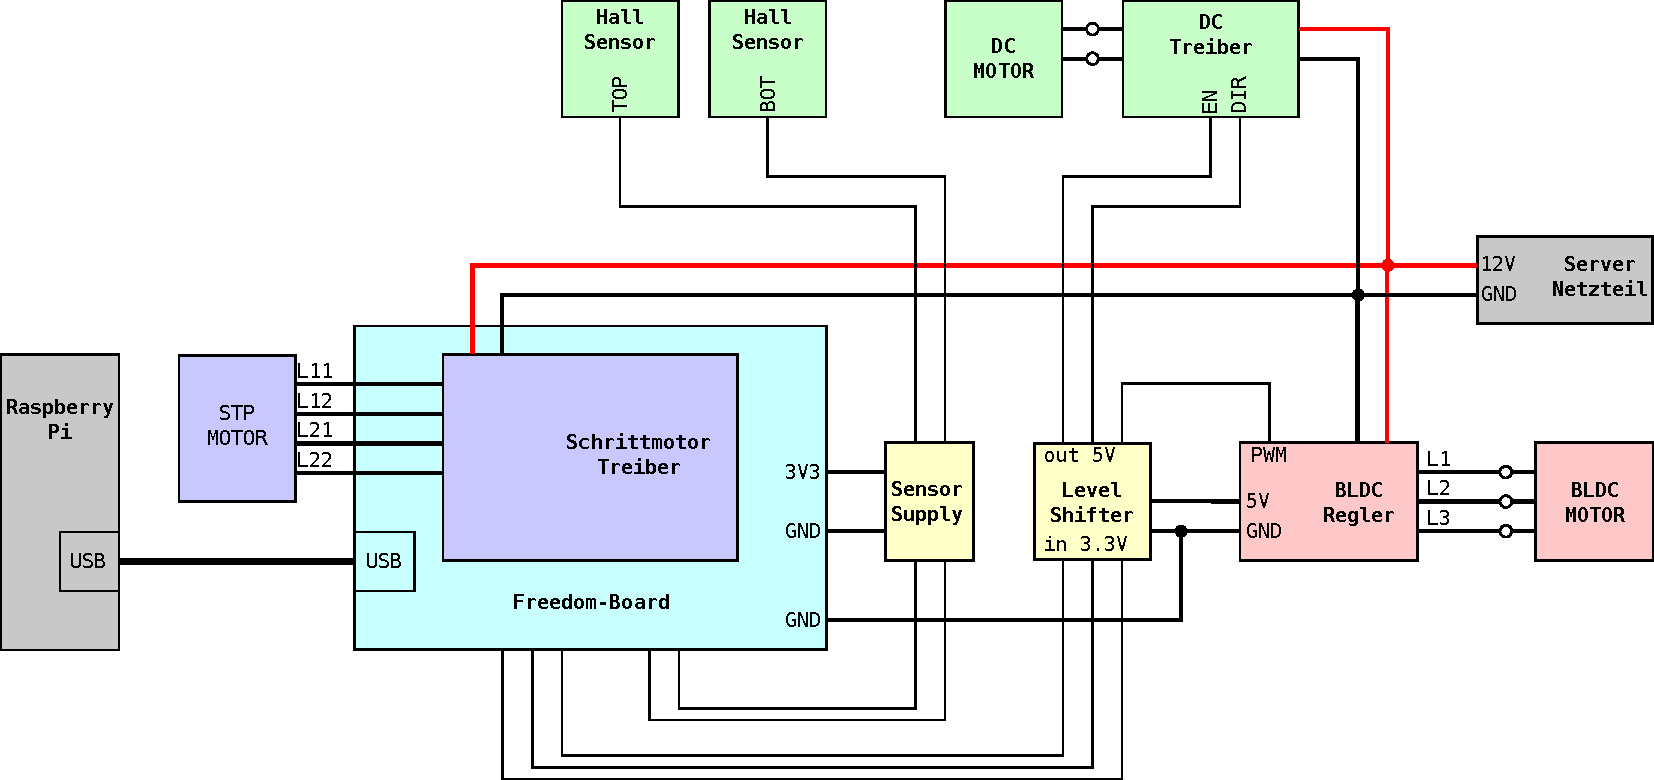
\includegraphics[width=0.95\textwidth]{../../fig/blockdiagram.pdf}
	\caption{Blockschaltbild der Elektrokomponenten}
	\label{fig:et-block}
\end{figure}

\newpage
\subsubsection{Speisung}

Die Speisung ist mehrstufig realisiert. Zum einen gibt es eine Speisung
welche die Energie für die Logikeinheiten liefert. Diese wird per Netzadapter
an das Raspberry Pi geführt. Dieses bildet die High-Level-Logik und somit die
zentrale Einheit welche eine 5 Volt Speisung zur Verfügung stellt an den
USB-Schnittstellen des Einplatinencomputers. Das Raspberry Pi wird per
USB-Kabel mit dem Freedomboard verbunden, über welches nebst den
Datenleitungen auch die Speisung geführt wird. So ist sichergestellt,
dass beide Einheiten eine gemeinsame Speisung haben welche auch der
logischen Hierarchie folgt. Das Freedomboard selbst stellt eine weitere
Speisung bereit auf dem eigenen Logikpegel von 3.3 Volt. Die Abbildung
\ref{fig:et-block_logic} zeigt das Blockschaltbild mit ausgeblendeten
Einheiten welche nicht von der Logikspeisung betrieben werden.

\begin{figure}[h!]
	\centering
	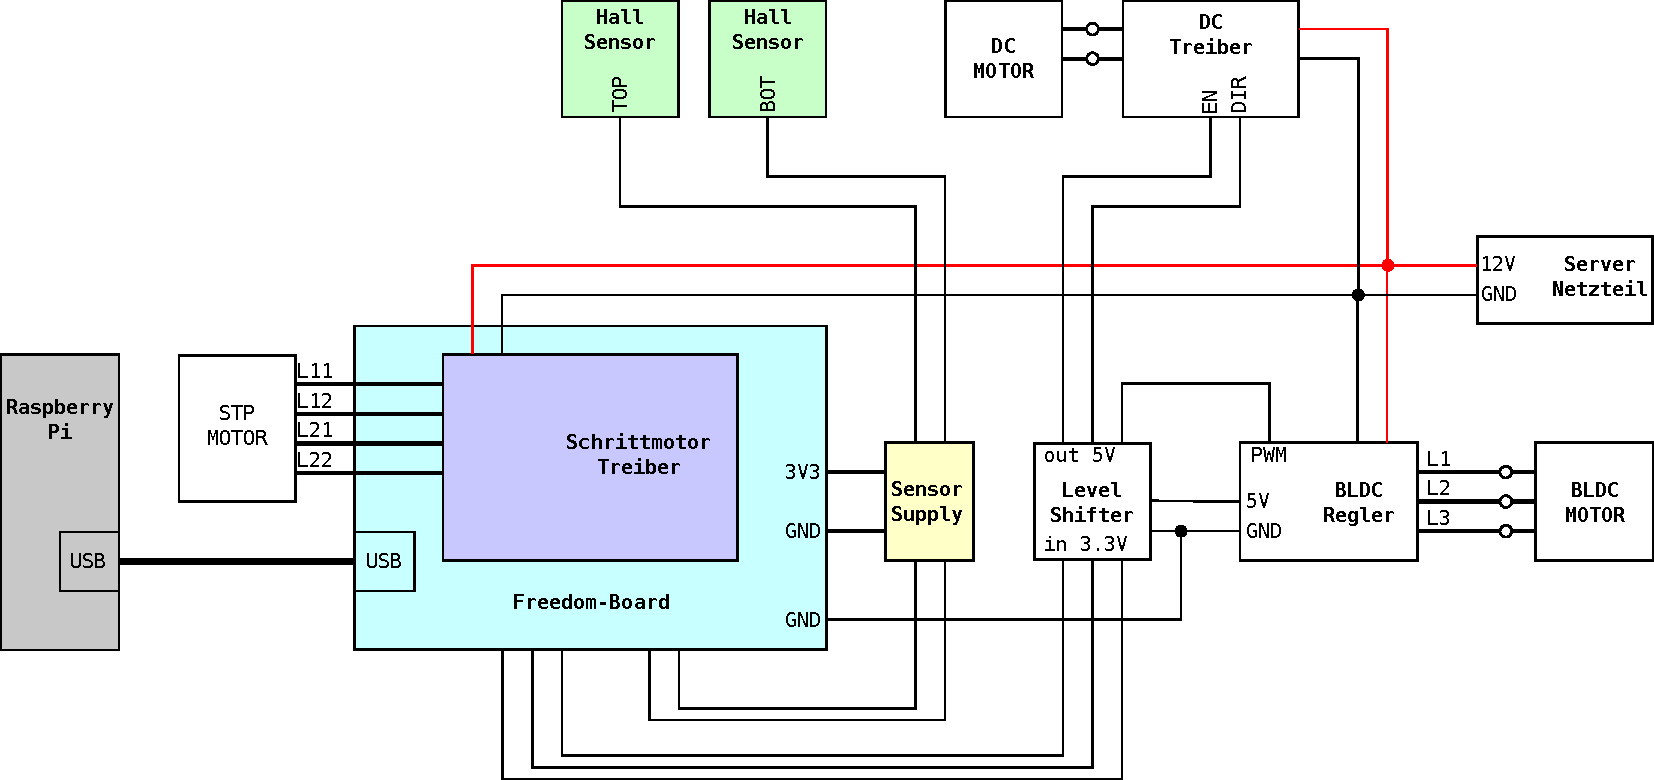
\includegraphics[width=0.95\textwidth]{../../fig/blockdiagram_logic.pdf}
	\caption{Blockschaltbild der Logikspeisung}
	\label{fig:et-block_logic}
\end{figure}

Nebst der Speisung für die Logik, welche auch die Kommunikation zwischen
Raspberry Pi und Freedomboard ermöglicht, bedarf es auch einer
Leistungsspeisung. Diese wird mittels eines Servernetzteils zur Verfügung
gestellt. Das Servernetzteil bietet eine 12 Volt Speisung welche für sämtliche
Motoren eingesetzt wird. Auf diese Weise kann eine satte Speisung
gewährleistet werden welche auch für höhere Leistungsänderungen fähig ist.
Nebst den Motoren und den zugehörigen Treibern wird auch der 3.3 Volt zu 
5 Volt Pegelwandler durch die Leistungsspeisung betrieben. Hierzu wird der
interne 5 Volt Spannungsregler der Brushlessansteuerung genutzt, welcher durch
die Leistungsspeisung betrieben wird. Dies garantiert stabile Pegel für die
Ansteuerung des Brushlessreglers so wie dies im beabsichtigen Einsatz
vorgesehen ist.




\newpage
\subsubsection{BLDC-Motor}
Der Antrieb für den Ballabwurf ist realisiert mittels eines
Brushless-Gleichstrommotors vom Modell A20-12XL EVO von Hacker.
Dieser wird mittels eines passenden kommerziellen Reglers vom
Typ X-30 PRO betrieben. Der Regler wird gestellt durch die Firmware
des Freedomboards, welche per UART bedient wird.

Die zugehörige Software kann mittels des UART-Interfaces per
Kommandozeile bedient werden mit dem Befehl \verb!BLDC! und den
zugehörigen Parametern. Die komplette Liste aller Befehle zu
\verb!BLDC! kann mittels \verb!BLDC help! aufgerufen werden.

\begin{figure}[h!]
	\centering
	\begin{subfigure}[b]{0.45\textwidth}
		\centering
		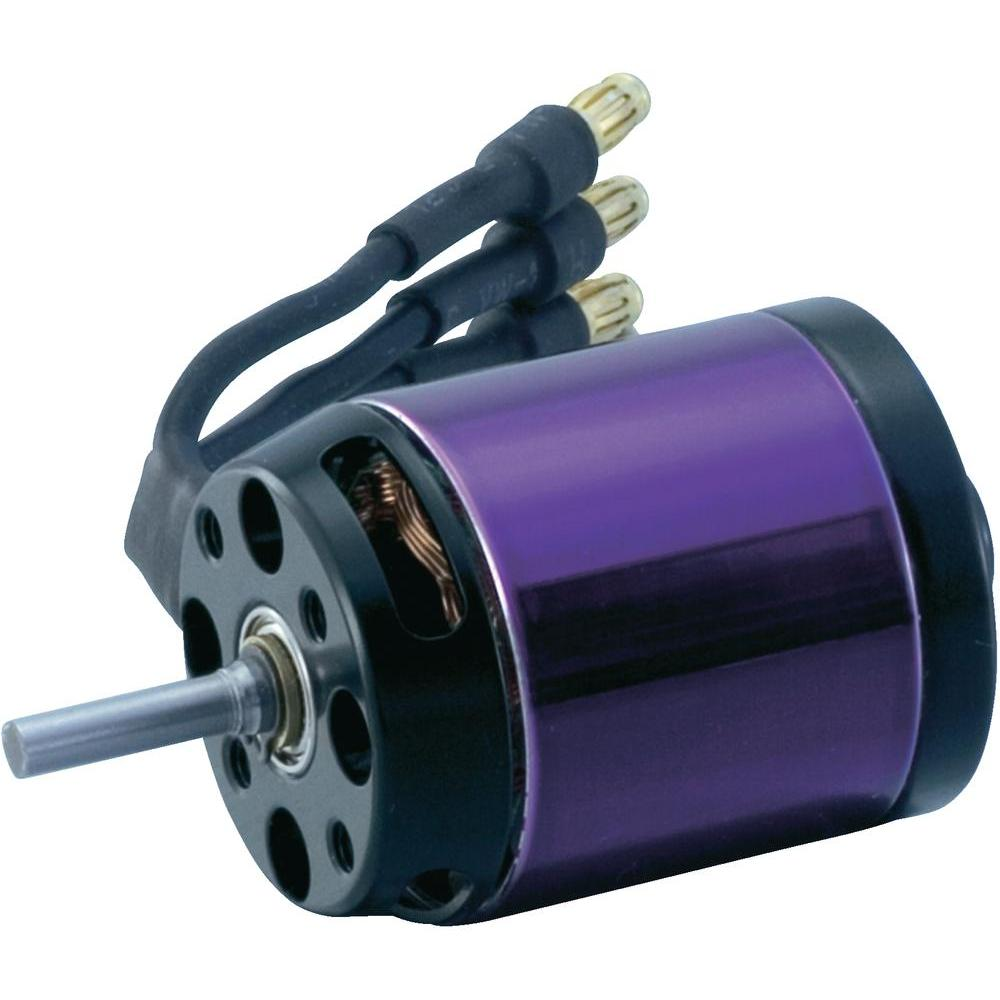
\includegraphics[width=0.75\textwidth]{../../fig/et/a20_12xl_evo.jpg}
		\caption{BLDC-Motor Hacker A20-12XL EVO}
	\end{subfigure}
	\begin{subfigure}[b]{0.45\textwidth}
		\centering
		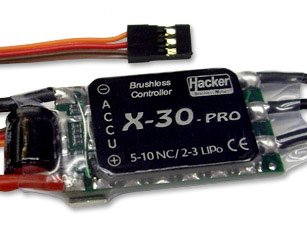
\includegraphics[width=0.75\textwidth]{../../fig/et/x30_pro.jpg}
		\caption{BLDC-Motor Hacker X-30 PRO}
	\end{subfigure}
	\caption{Antriebssystem für den Ballabwurf}
\end{figure}

Da ein kommerzieller Regler verwendet wird aus dem Modellbau für
Flugzeuge und Helikopter, kann lediglich ein Standard PWM-Signal
aus dem Modellbau benutzt werden, um die Drehzahl des Motors zu
stellen. Da dieser Regler eine echte Drehzahlregelung implementiert
wird auf einen überlagerten Regler auf dem Freedomboard verzichtet.
Eine allfällige Parametierung kann mittels eines Programmieradapters
X-PRO USB Controller V2 des Herstellers vorgenommen werden.

%\input{content/et/nachschub}
%\input{content/et/ausrichtung}

% \subsubsection{Übersicht}
% Die Elektronik ist organisiert in einem modularen Verbund von verschiedenen
% Funktionsgruppen. Nebst den elementaren Einheiten wie Motoren und zugehörigen
% Treibern gehören auch etwa Pegelwandler und Sensoren dazu. Die Abbildung
% \ref{fig:et-block} zeigt schematisch den Zusammenhang dieser Komponenten.
% 
% 
% \begin{figure}[h!]
% 	\centering
% 	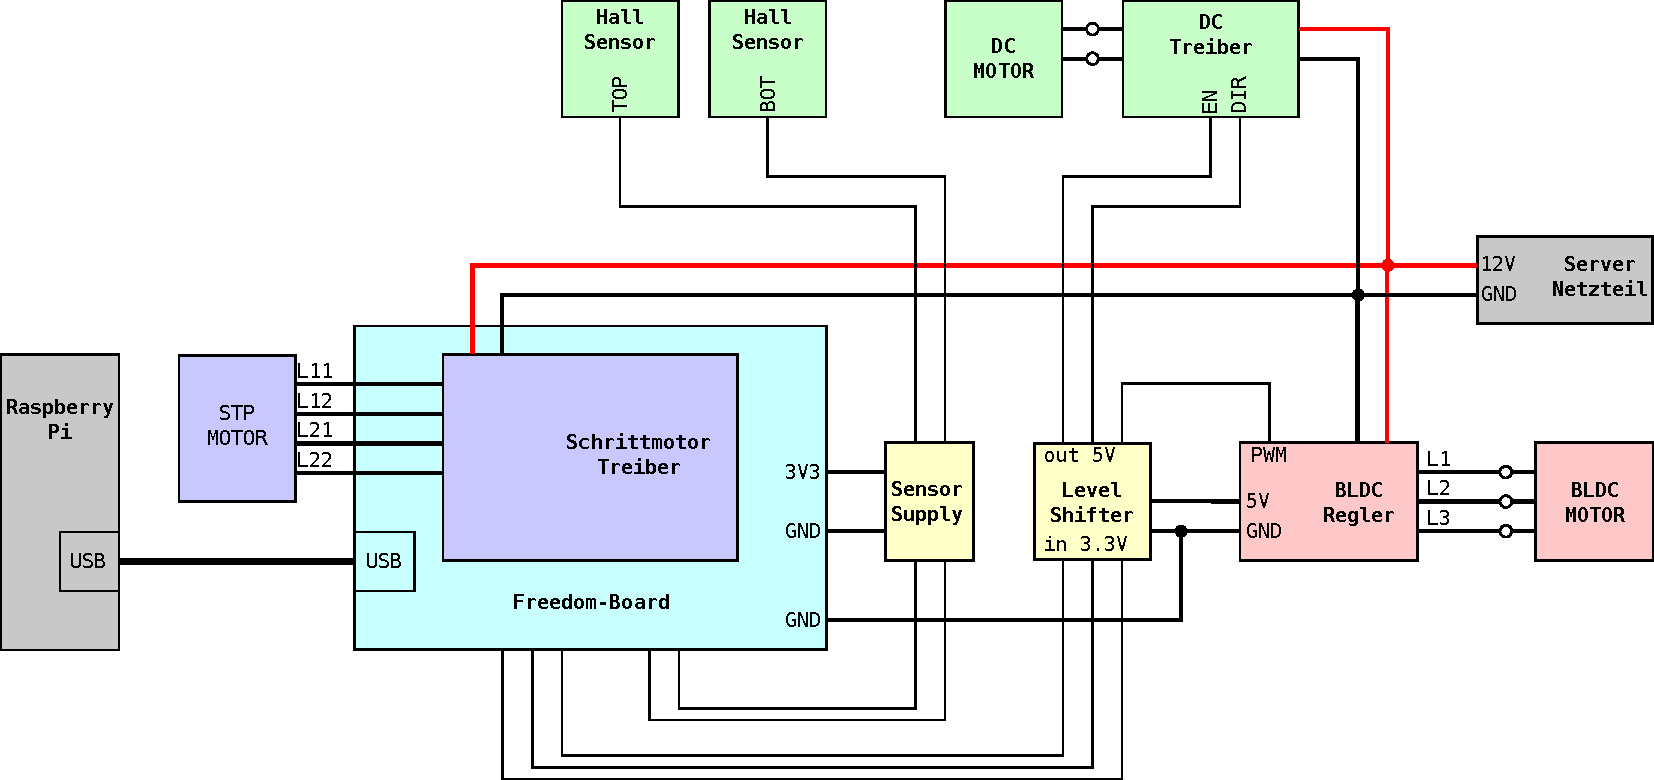
\includegraphics[width=0.95\textwidth]{../../fig/blockdiagram.pdf}
% 	\caption{Blockschaltbild der Elektrokomponenten}
% 	\label{fig:et-block}
% \end{figure}
% 
% \newpage
% \subsubsection{Speisung}
% 
% Die Speisung ist mehrstufig realisiert. Zum einen gibt es eine Speisung
% welche die Energie für die Logikeinheiten liefert. Diese wird per Netzadapter
% an das Raspberry Pi geführt. Dieses bildet die High-Level-Logik und somit die
% zentrale Einheit welche eine 5 Volt Speisung zur Verfügung stellt an den
% USB-Schnittstellen des Einplatinencomputers. Das Raspberry Pi wird per
% USB-Kabel mit dem Freedomboard verbunden, über welches nebst den
% Datenleitungen auch die Speisung geführt wird. So ist sichergestellt,
% dass beide Einheiten eine gemeinsame Speisung haben welche auch der
% logischen Hirachie folgt. Das Freedomboard selbst stellt eine weitere
% Speisung bereit auf dem eigenen Logikpegel von 3.3 Volt. Die Abbildung
% \ref{fig:et-block_logic} zeigt das Blockschaltbild mit ausgeblendeten
% Einheiten wleche nicht von der Logikspeisung betrieben werden.
% 
% \begin{figure}[h!]
% 	\centering
% 	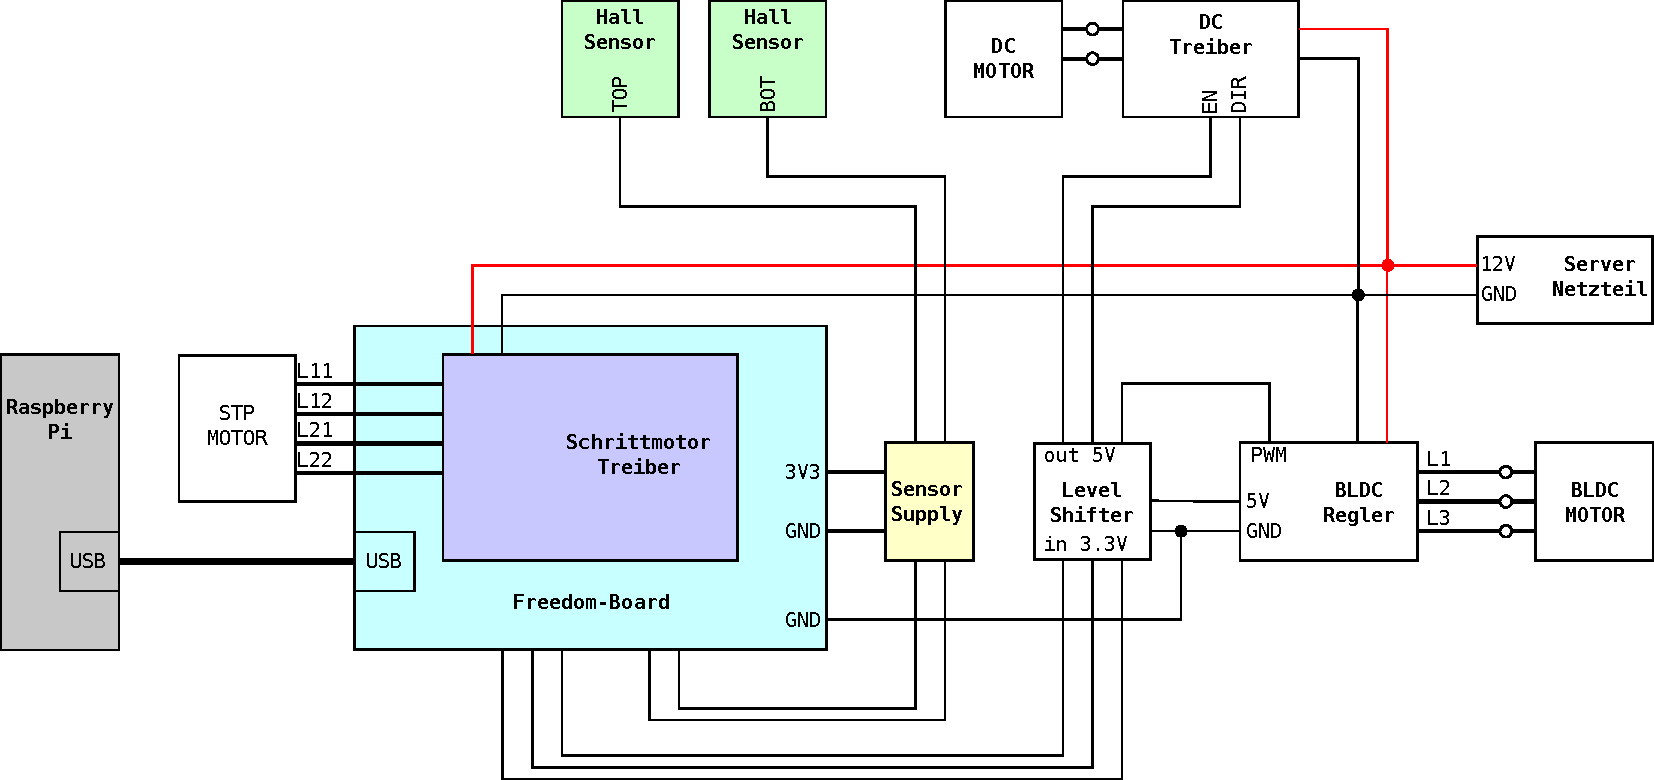
\includegraphics[width=0.95\textwidth]{../../fig/blockdiagram_logic.pdf}
% 	\caption{Blockschaltbild der Logikspeisung}
% 	\label{fig:et-block_logic}
% \end{figure}
% 
% Nebst der Speisung für die Logik, welche auch die Komminukation zwischen
% Raspberry Pi und Freedomboard ermöglicht, bedarf es auch einer
% Leistungsspeisung. Diese wird mittels eines Servernetzteils zur Verfügung
% gestellt. Das Servernetzteil bietet eine 12 Volt Speisung welche für sämtliche
% Motoren eingesetzt wird. Auf diese Weise kann eine satte Speisung
% gewährleistet werden wleche auch für höhere Leistungsänderungen fähig ist.
% Nebst den Motoren und den zugehörigen Treibern wird auch der 3.3 Volt zu 
% 5 Volt Pegelandler durch die Leistungsspeisung betrieben. Hierzu wird der
% interne 5 Volt Spannungsregler der Brushlessansteuerung genutzt, welcher durch
% die Leistungsspeisung betrieben wird. Dies garantiert stabile Pegel für die
% Ansteuerung des Brushlessreglers so wie dies im beabsichtigen Einsatz
% vorgesehen ist.




\newpage
\newpage
\section{Projektmanagement}

\begin{figure}[h!]
	\centering
	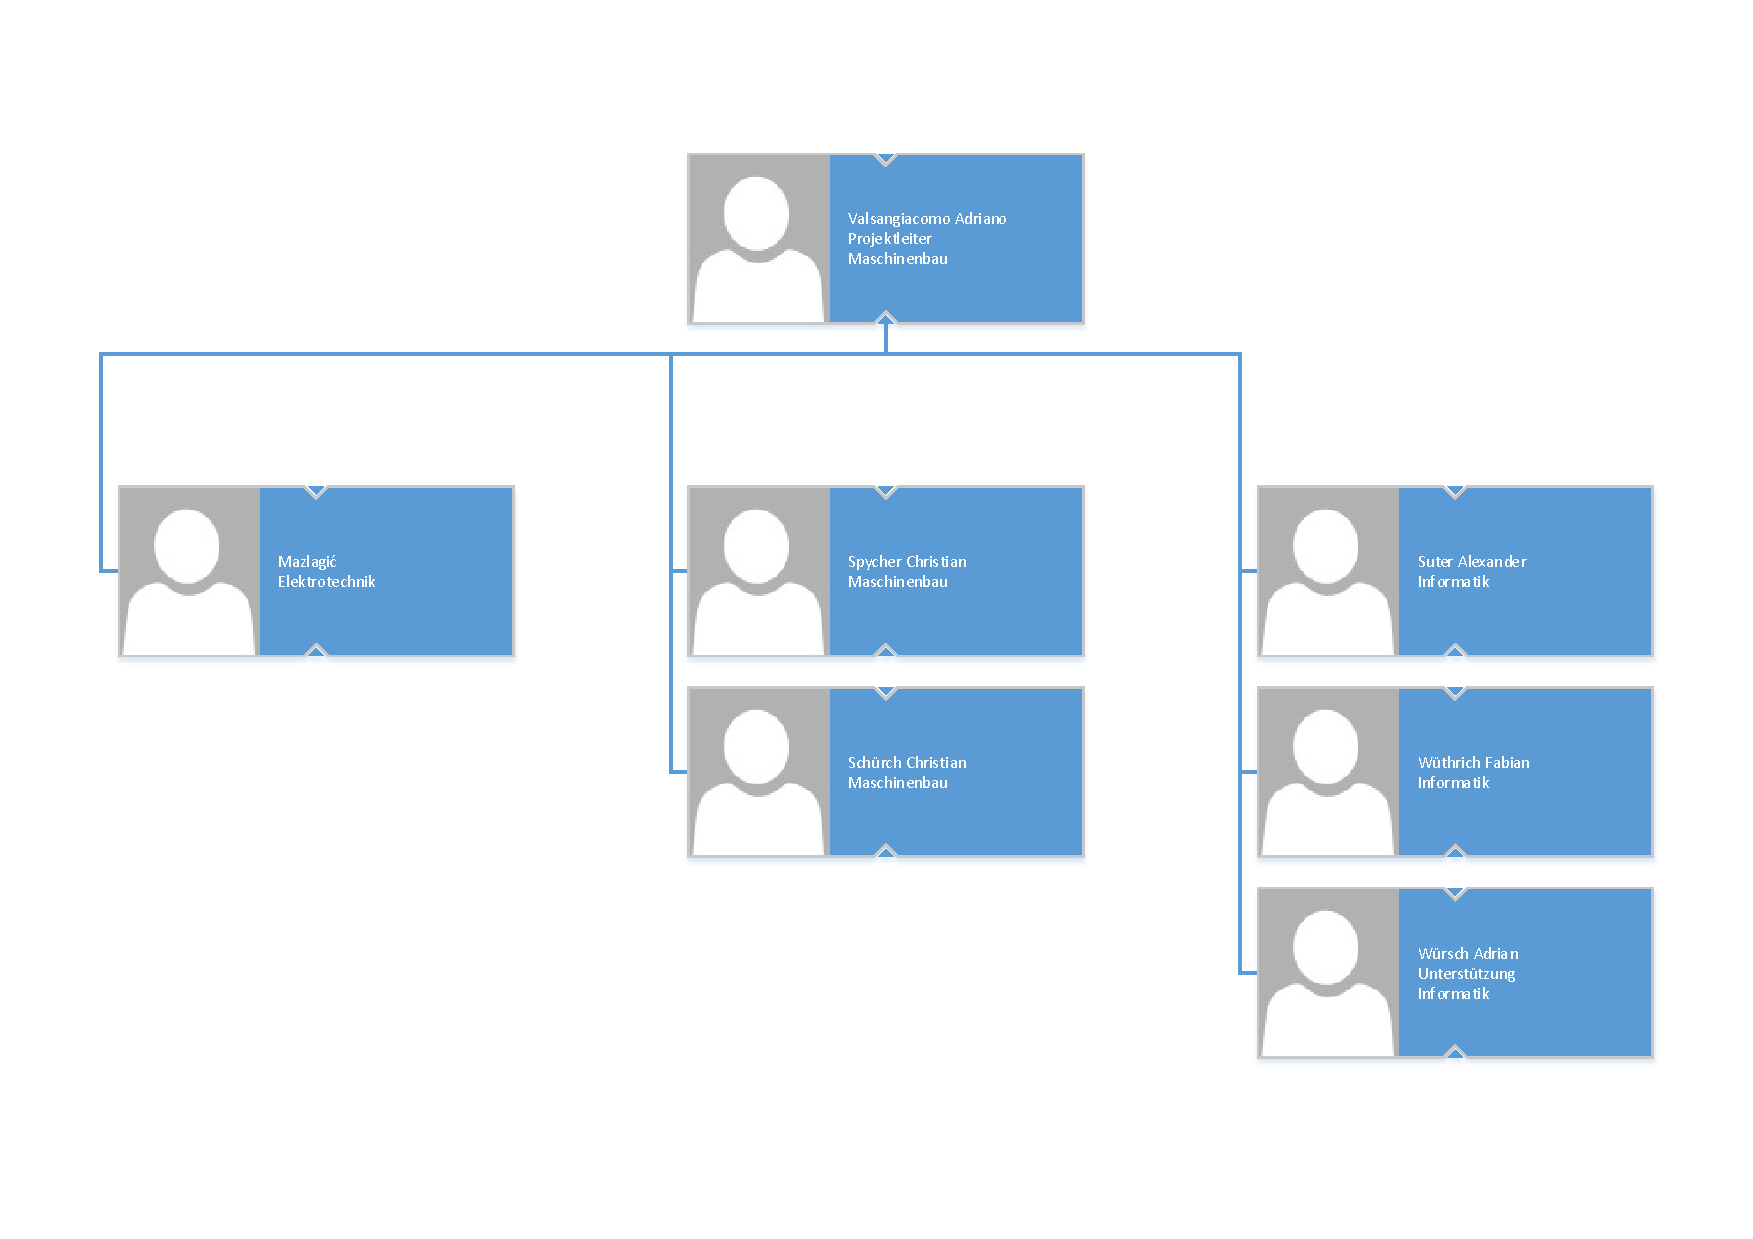
\includegraphics[width=1.0\linewidth]{../../fig/Organigramm.pdf}
	\caption{Organisation der Gruppe}
	\label{fig:Organigramm}
\end{figure}

\noindent
Die Projektführung wurde von Adriano Valsangiacomo durchgeführt. Er
koordinierte die einzelnen Teilgruppen und sorgte für Reibungslosen
Betrieb. Adrian Würsch, als neues Mitglied, wurde der Informatik
zugeteilt. Dort führte er unterstützende Arbeiten aus.

\subsection{Grobplanung}
In der Grobplanung wurden die wichtigsten Meilensteine des Gesamtsystems und der einzelnen Disziplinen festgehalten.
Der Zeitstrahl in Abbildung \ref{fig:rahmenplanung} zeigt die chronologische Reihenfolge an. Als klar wurde, dass die Umsetzung in Verzug war, wurde die Planung angepasst. Vorallem im Bereich der Elektrotechnik wurde der Engpass ersichtlich. Wir waren uns bewusst, dass es dort zu Verzögerungen kommen kann, da dieser Bereich mehr oder weniger eine one-man-show ist. Darum wurden im ET Bereich zuerst Arbeiten erledigt, welche Abhängigkeiten mit anderen Disziplinen hatten.

\subsubsection{Stand 19.02.2015}
Der Rahmenplanung sind die wichtigsten Termine zu entnehmen. Dies sind drei offizielle Termine wie diverse kleinere, welche jeweils von den Disziplinen selbst für sich gesetzt wurden. Der erste Meilenstein wurde auf den 6. März datiert, dort soll sich das Team über die Planung und Umsetzung sicher sein.
Meilenstein zwei wurde auf den 10. April festgelegt, mit dem Ziel die Maschine fertig montiert zu haben. Eine Woche später sollte anschliessend die Tests beginnen. Die lauffähige und getestete Maschine und zugleich 80\% der Dokumentation bildeten zusammen Meilenstein 3.

\begin{figure}[h!]
	\centering
	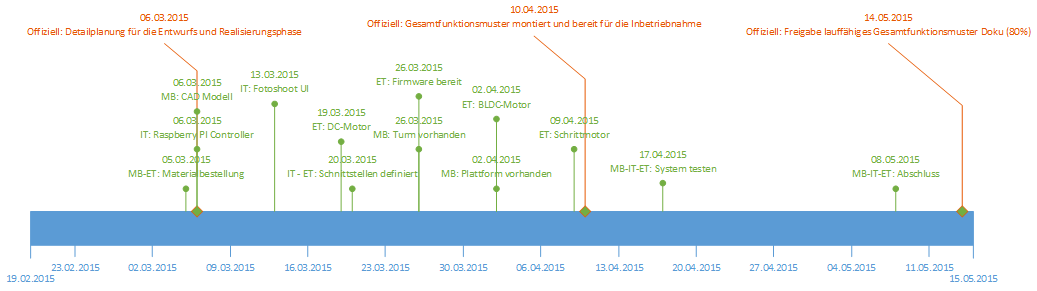
\includegraphics[width=1\linewidth]{../../fig/rahmenplanung}
	\caption{Rahmenplan vom 19.02.2015}
	\label{fig:rahmenplanung}
\end{figure}

\newpage
\subsubsection{Stand: 10.04.2015}
Am 10.04.2015 hat sich das Team zusammengeschlossen um über die restlichen Arbeiten zu diskutieren. Darauf hin hat man sich entschlossen die restliche Planung anzupassen. Nun wurden teilweise neue Termine definiert, welche für den restlichen Verlauf bindend sind.

\begin{figure}[h!]
	\centering
	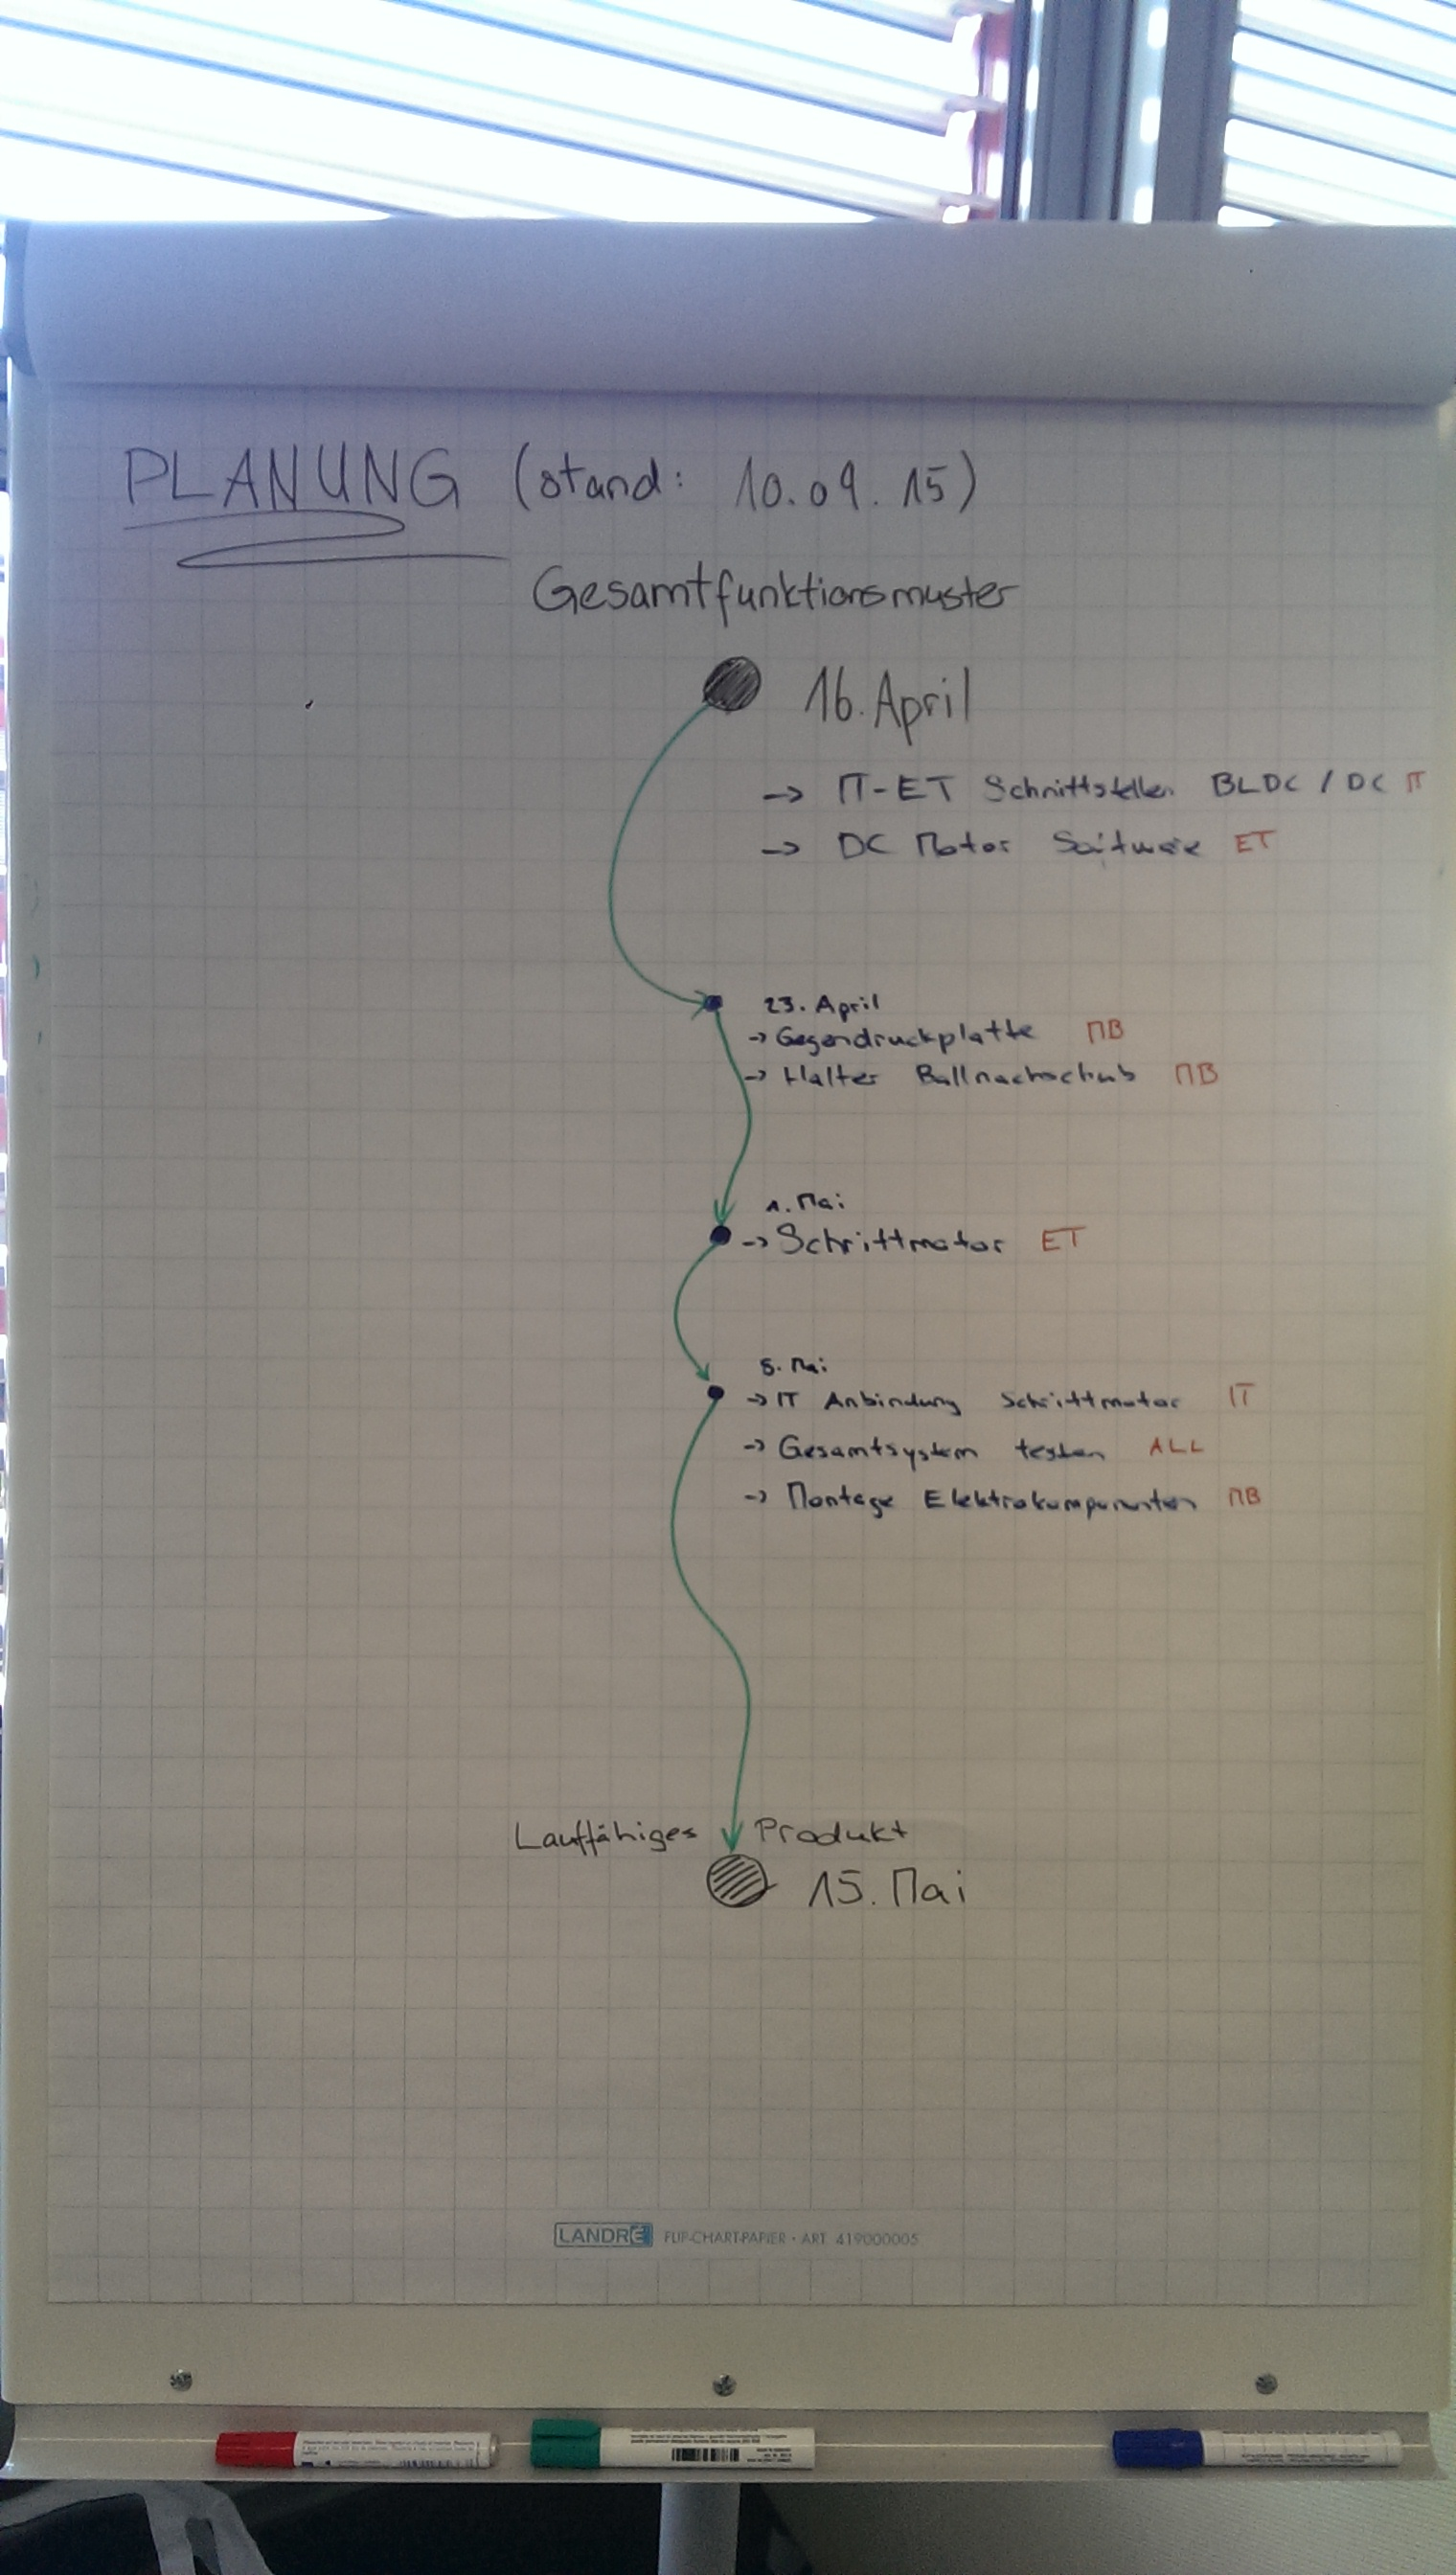
\includegraphics[width=0.6\linewidth]{../../fig/rahmenplanung-10042015}
	\caption{Rahmenplan vom 10.04.2015}
	\label{fig:rahmenplanung-10042015}
\end{figure}



\newpage
\subsection{Projektkosten}
Dem Projekt wurden 600.00 Franken zur Verfügung gestellt. In der Summe wurden 486.70 Franken davon verwendet. In der Grafik \ref{fig:kostenuebersicht} sind alle Komponenten aufgelistet.

\begin{figure}[h!]
	\centering
	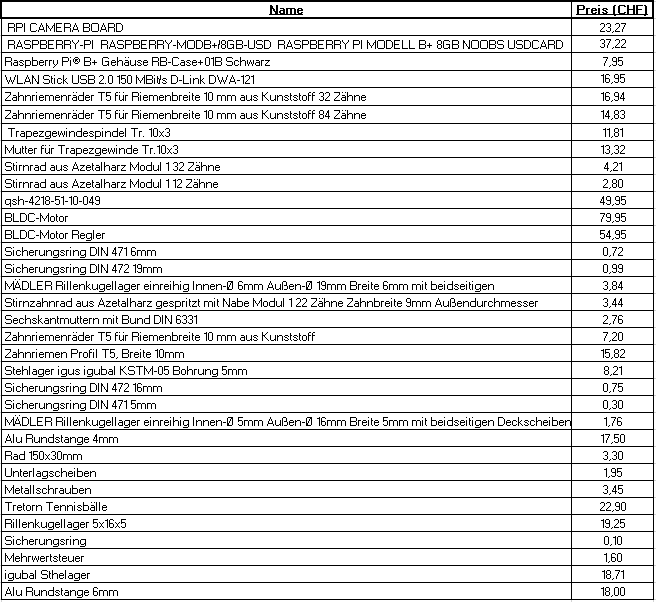
\includegraphics[width=\linewidth]{../../fig/Kosten}
	\caption{Kostenübersicht}
	\label{fig:kostenuebersicht}
\end{figure}

\newpage
\subsection{Projektrisiko}

Im Team wurden Projektrisiken evaluiert und anhand der Wahrscheinlichkeit und der entstehenden Auswirkung eingeordnet. Zusätzlich wurden Gegenmassnahmen beschrieben.

\begin{table}[h!]
	\centering
	\begin{tabular}{r || c c c c}
		häufig 		
		& \cellcolor{red} 
		& \cellcolor{red}
		& \cellcolor{red}
		& \cellcolor{red} \\
		wahrscheinlich		
		& \cellcolor{yellow} 
		& \cellcolor{yellow} 
		& \cellcolor{red}
		& \cellcolor{red} \\
		gelegentlich		
		& \cellcolor{yellow}
		& \cellcolor{yellow}
		& \cellcolor{yellow}
		& \cellcolor{red} \\
		vorstellbar		
		& \cellcolor{green}
		& \cellcolor{yellow}
		& \cellcolor{yellow}
		& \cellcolor{yellow} \\
		unwahrscheinlich	
		& \cellcolor{green}
		& \cellcolor{green}
		& \cellcolor{yellow}
		& \cellcolor{yellow} \\
		unvorstellbar		
		& \cellcolor{green}
		& \cellcolor{green}
		& \cellcolor{green}
		& \cellcolor{green} \\
		\hline
		& unwesentlich & geringfügig & kritisch & katastrophal
	\end{tabular}
	\caption{Risikoreferenz}
	\label{tab:risikoreferenz}
\end{table}


\begin{landscape}
	\begin{table}
		\begin{tabular}{|p{5cm}|c|c|p{9cm}|}
			\hline Risiko & Auswirkung & Wahrscheinlichkeit & Massnahmen \\ 
			
			\hline \rowcolor{yellow} IT, MB Projektmitglied fällt aus & geringfügig & vorstellbar & 
			- Vorzeitig über Abwesenheit informieren \newline
			- Arbeitsstand in Gruppe kommunizieren \\ 
			
			\hline \rowcolor{red} ET Projektmitglied fällt aus & katastrophal & gelegentlich & 
			- Wöchentlicher Gesundheits- und Gemütszustand rapportieren \newline
			- Aufbau Know-How in den ET Arbeiten \\
			
			\hline \rowcolor{yellow} \hline Abweichung vom Terminplan & geringfügig & vorstellbar &
			- Realistische Planung \newline
			- Aufarbeiten in Reservezeit \\ 
			
			\hline \rowcolor{yellow} \hline Fehlende Zuverlässigkeit & kritisch & unwahrscheinlich &
			- Klare Aufgabenverteilung \newline
			- Review durch Teammitglieder \\ 
			
			\hline \rowcolor{yellow} \hline Algorithmus zur Korberkennung nicht robust & kritisch & vorstellbar &
			- Gutes Unit-Testing des Algorithmus \newline
			- Früh implementieren und testen \\
			
			\hline \rowcolor{green} \hline Fehlendes Know-How IT & geringfügig & unwahrscheinlich &
			- RaspyPi früh aufsetzen \newline
			- Know-How in Python aufbauen \\ 
			
			\hline \rowcolor{yellow} \hline Integration der ET Schnittstellen in die IT Umgebung & geringfügig & wahrscheinlich &
			- Schnittstellen definieren  \\
			
			\hline \rowcolor{yellow} \hline Bälle treffen nicht präzise & kritisch & vorstellbar &
			- Früh testen \newline
			- Ballanpressdruck variieren \\ 
			
			\hline \rowcolor{yellow} \hline Stabilität beim Abwurf & kritisch & vorstellbar &
			- Mehr Gewicht montieren oder Seitenstütze \newline
			- Dicke der Wände \\ 
			
			\hline \rowcolor{yellow} \hline Falsche Dimensionierung der Motoren & kritisch & vorstellbar &
			- Motoren neu kaufen. \\
			
			\hline \rowcolor{yellow} \hline Energieversorgung: Umbau von Servernetzteilen gelingt nicht & kritisch & vorstellbar &
			- Andere Energieversorgung wählen \\ 
			
			\hline \rowcolor{yellow} \hline Schwingungen beim Abwurf & kritisch & vorstellbar &
			- Drehrad auswuchten \newline
			- Drehzahl reduzieren \newline
			- Konstruktion verstärken \\
			
			\hline \rowcolor{green} \hline Budget & geringfügig & unwahrscheinlich &
			- Budgetplanung laufend aktualisieren  \newline 
			- Planen bevor etwas eingekauft wird \\
			
			\hline \rowcolor{yellow} \hline Achse BLDC nicht stark genug & katastrophal & vorstellbar &
			- Lagerung auf der gegenüberliegenden Seite des Motors erstellen \newline
			- Trägheitsmoment Wurfrad anpassen \newline
			- Langsameres anfahren \\
			
			\hline \rowcolor{yellow} \hline BLDC überhitzt & kritisch & vorstellbar &
			- BLDC nicht im Dauerbetrieb laufen lassen \newline
			
			
			
		\end{tabular}
		\caption{Risikomanagement}
		\label{tab:risikomanagement}
	\end{table} 
\end{landscape}
\newpage
\newpage
\section{Schluss}

Im PREN1 wurden Grobkonzepte und Lösungsvorschläge erarbeitet. Im PREN2 durfte das ausgewählte Konzept \textit{Drehrad} umgesetzt werden. Das Team setzte sich zusammen und definierte wie die Umsetzung durchgeführt werden soll. Anschliessend konnte endlich mit der praktischen Arbeit gestartet werden. In Zusammenarbeit wurden die Disziplin übergreifenden Schnittstellen definiert. Wie gross ist das Raspberry-Pi? Wo darf es platziert werden? Wie viel Kraft benötigt der Schrittmotor? Wie schwer sind die Elektrotechnik Komponenten? All diese Fragen und noch viele weitere wurden während der Umsetzung gestellt und gelöst.

Nach wenigen Wochen konnten die ersten Teile zusammengesetzt werden. Wie zu erwarten, funktionierte nicht alles einwandfrei. Die gesamte Maschine konnte optimiert werden um den geforderten Erwartungen zu entsprechen. Zusätzliche Anforderungen für das Testing wurden erst während des Projektes Team-Intern definiert. So wollte man beispielsweise, dass die einzelnen Motoren per Knopf-Druck auf dem Notebook gestartet und gestoppt werden können. So entstand teilweise in der Informatik zusätzlicher Aufwand, welcher jedoch zu keinen zeitlichen Verzögerungen führte.

Durch seriöses Projektmanagement konnten alle Korrekturen überwacht und abgesprochen werden. So konnte frühzeitig reagiert werden, falls ein Ziel nicht oder verspätet erreicht wurde. Das Projekt konnte durch die engagierte Mitarbeit aller Beteiligten erfolgreich abgeschlossen werden.

\subsection{Lessons learned}

Das ganze Team konnte im letzten Jahr wertvolle Erfahrungen sammeln. Nachfolgend einige Punkte, welche wir besonders hervorheben möchten:

\begin{enumerate}
	\item  In einem interdisziplinären Projekt steht die \textbf{Zusammenarbeit} an oberster Stelle. Arbeitet eine Disziplin im Elfenbeinturm, dann wird ein erfolgreicher Projektabschluss schwierig.
	\item Schnittstellen-Definitionen sollten möglichst früh definiert werden, damit jeder weiss, was für Anforderungen die Komponente zu erfüllen hat. Auch benötigte Änderungen dieser Definitionen müssen schnell und klar \textbf{kommuniziert} werden.
	\item Möglichst schnell in die Komponenten-\textbf{Tests} einsteigen. Umso früher integrierte Komponenten getestet werden können, umso früher wird erkannt, was funktionieren kann und was nicht. Uns wurde so relativ schnell klar, dass die Konstruktion für die Ballführung verbessert werden muss, damit diese nicht blockiert.
	\item \textbf{Risiken} können sich ändern. Wurde zu Beginn die Ortung des Korbes als grosses Risiko wahrgenommen, weil Know-How in diesem Bereich vermisst wurde. Zeichnete sich ab, dass der Wurf-Mechanismus einige Risiken mehr mit sich brachte.
\end{enumerate}

\subsection{Würdigung}
Das PREN Team 39 bedankt sich bei allen Personen, welche einen Teil zum Projekt beigetragen haben. Ein besonderer Dank geht an den Projektbetreuer Herr \textbf{Martin Vogel}, welcher durch energisches Hinterfragen unserer Lösung einen wichtigen Teil zum Erfolg unseres Projektes beigetragen hat. Ein Teammitglied ist besonders hervorzuheben. Die Elektrotechnik war mit nur einem Mann schwach besetzt, hatte jedoch mit der Ansteuerung von drei Motoren enorm viel Aufwand. Die restlichen Teammitglieder bedanken sich bei \textbf{Ervin} für seinen unermüdlichen Einsatz.
\newpage

%Anhang
\appendix
\section{Aufgabenstellung}

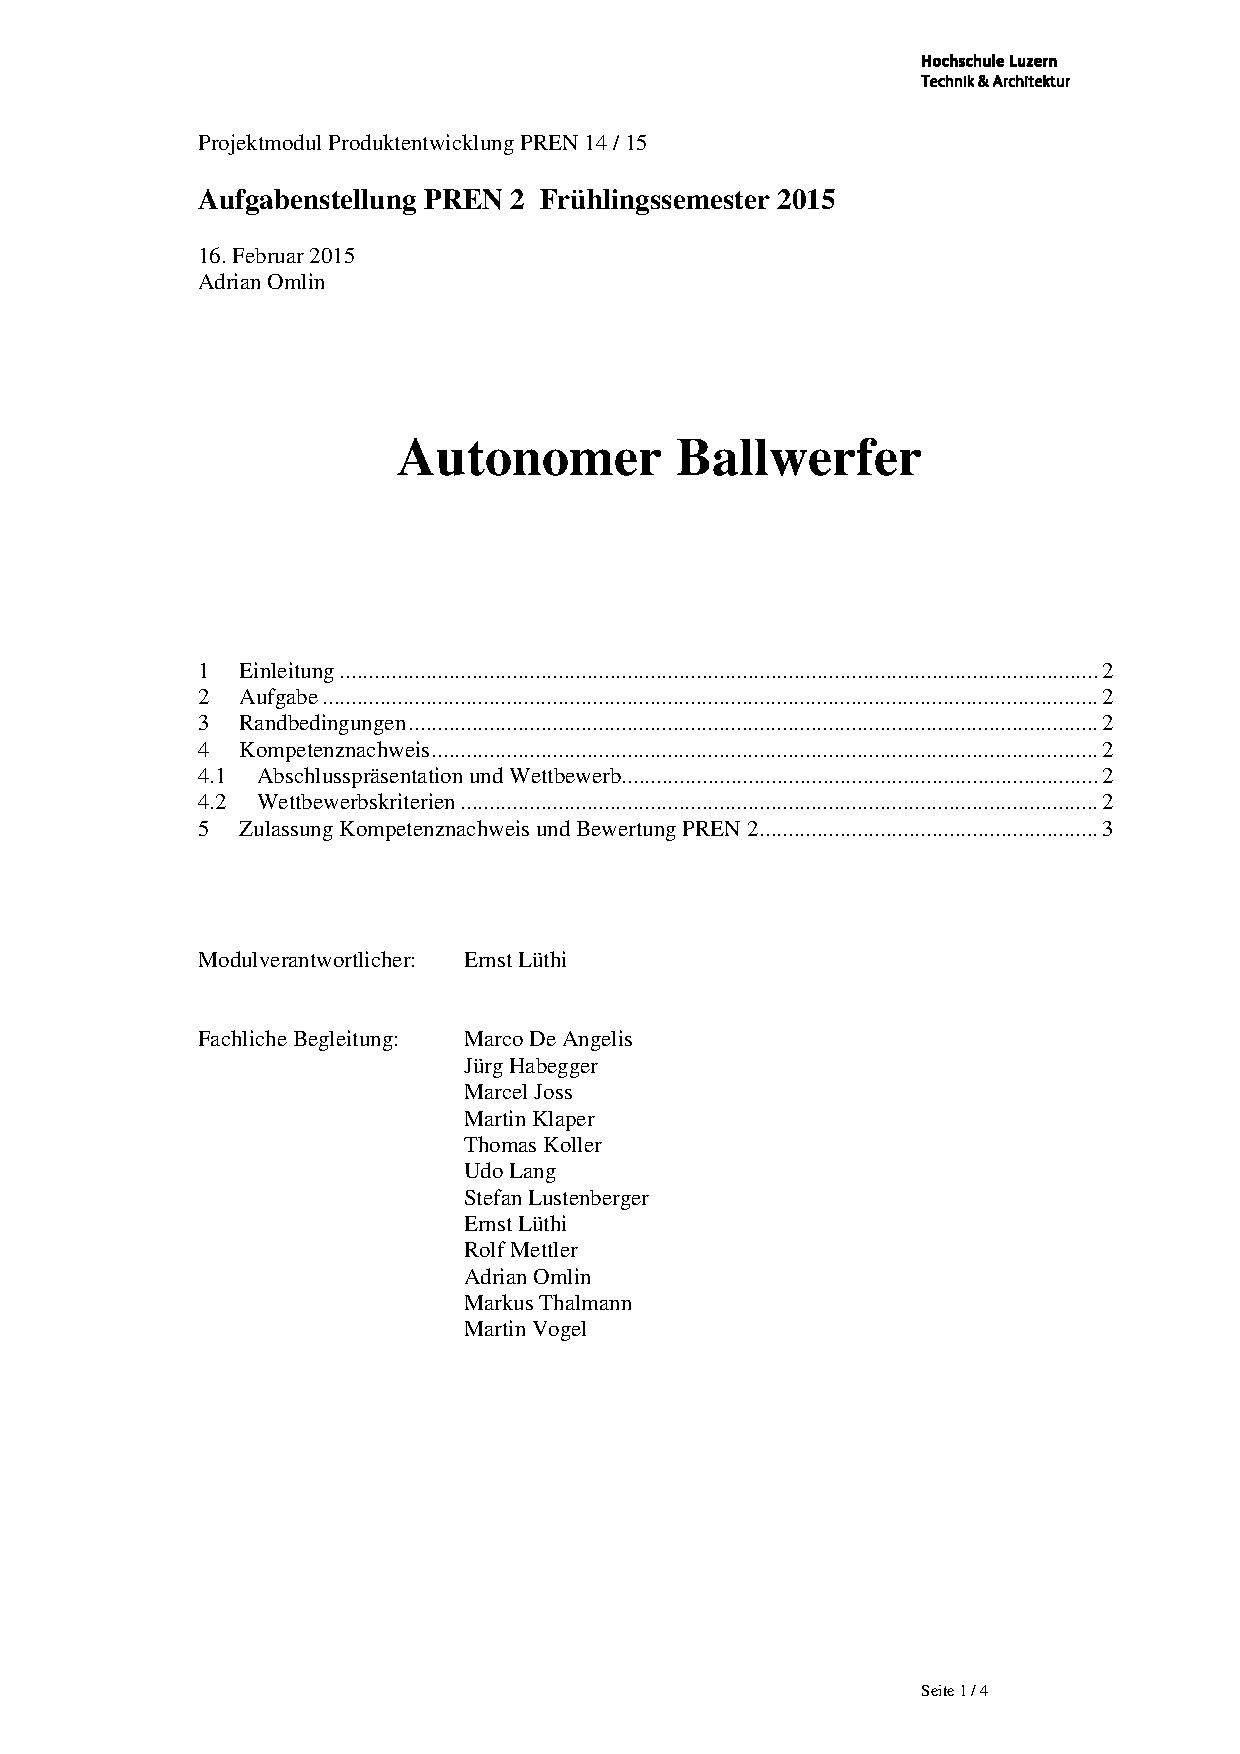
\includepdf[pages=-,offset=0 -2.2cm,frame,width=0.92\textwidth,picturecommand={\centering},pagecommand={\thispagestyle{fancy}},]{../../fig/Aufgabenstellung_PREN2_F15.pdf}
\newpage
\section{Technologierecherche}


\includepdf[pages=-,offset=0 -2.2cm,frame,width=0.92\textwidth,picturecommand={\centering},pagecommand={\thispagestyle{fancy}},]{../../fig/Team_39_Technologierecherche.pdf}
\newpage
\section{Produktanforderungen}
\label{sec:produktanforderungen}

Die Anforderungen wurden vom Team im PREN1 definiert und durch den betreuenden Dozenten abgenommen. Im Verlaufe des PREN2 wurden die Anforderungen angepasst und durch den Dozenten bestätigt. Nachfolgend liegt die vollständige Anforderungsliste vor. Auf der Liste ist erkennbar, welche Anforderungen geändert wurden. Nicht mehr gültige Anforderungen sind \sout{durchstrichen} und neue Elemente sind \uline{unterstrichen}.

\renewcommand{\arraystretch}{1.5}
\begin{longtable}[l]{|l|c|l|p{8.5cm}|}
	\hline
	\textbf{Nr.} & \textbf{F/M/W} & \textbf{Bezeichnung} & \textbf{Wert/Daten/Erläuterungen} \endhead
	
	\hline 1 &  & Gerät & \\ 
	\hline 1.1 & F & Gerätemasse & 0.5 m $\times$ 0.5 m $\times$ 1.0 m  \\
	\hline 1.2 & M & Gewicht & < 8 kg (ohne Energieversorgung, Tennisbälle und externes Kommunikationsgerät) sonst 0 Punkt \\
	\hline 1.3 & W & Gewicht & \sout{< 4 kg} \newline \uline{< 6 kg (Begründung: Gewählter Aufbau wird durch Motoren und Konstruktion schwerer)} \\
	\hline 1.4 & W & Standfestigkeit & stabil \\
	\hline 1.5 & F & Startbefehl & drahtlos über ein externes Kommunikationsgerät (\sout{Smartphone}, \sout{Tablet}, Computer) \newline \uline{Es wird lediglich eine Java-Applikation für das Notebook entwickelt. Die Zeit ist zu knapp um ein App zu entwickeln.} \\   
	\hline 1.6 & F & Stoppbefehl & auf demselben Kommunikationsgerät \sout{akustisch oder} visuell ausgegeben \newline \uline{Akustisch ist keine Pflicht, wenn es visuell ausgegeben wird. Akustisch wird somit nicht benötigt.}  \\ 
	\hline 1.7 & W & Kommunikationsgerät & \sout{App auf Smartphone} \newline \uline{App keine Pflicht. Die Applikation läuft auf dem Notebook. Der Zeitraum um eine App zu entwickeln ist zu klein.} \\
	\hline 1.8 & F & Aufhängevorrichtung & muss vorhanden sein (Wägen) \\
	\hline 1.9 & F & Selbstständigkeit & keine Eingriffe von aussen nach dem Start \\
	\hline 1.10 & W & Trefferquote & 100 \% (5 von 5 Bällen) \\
	\hline 1.11 & W & Prozesszeit & \sout{< 1 Min}. \newline
	\uline{< 90 Sekunden. Nachdem erkannt wurde, dass die Bilderkennung auf dem Raspberry PI nicht so rasant ist wie auf dem Notebook, sind wir mit der Zeit von 90 Sekunden zufrieden. Wichtiger ist die Stabilität und Funktionstüchtigkeit des Systems.} \\
	\hline 1.12 & M & Startpositionierung & von Hand mithilfe von Schablone \\
	\hline 2 &  & Energieversorgung & \\
	\hline 2.1 & W & Bauart & einfach zu entnehmen  \\
	\hline 2.2 & F & Bereitstellung & muss transportierbar sein  \\
	\hline 2.3 & W & Wirkungsgrad & hoch \\
	\hline 3 &  & Spielfeld & \\
	\hline 3.1 & F & Abmasse & siehe Aufgabenstellung \\       
	\hline 3.2 & F & Spielfeldrand & darf nicht umgriffen werden  \\
	\hline 3.3 & F & Zone ohne Hindernisse & 0.5 m $\times$ 0.5 m $\times$ 1.8 m um Spielfeldrand \\
	\hline 3.4 & F & Veränderungen am Spielfeld & keine erlaubt (z.B. Führungsschiene) \\
	\hline 3.5 & F & Begrenzungslinie & darf nicht überragen oder überfahren werden \\
	\hline 3.6 & F & Spielfeldboden & besteht aus hellen Spanplatten \\
	\hline 3.7 & F & Spielfeldrückwand & besteht aus hellen Spanplatten \\
	\hline 4 &  & Tennisball & \\
	\hline 4.1 & F & Gewicht & 55 g - 60 g  \\
	\hline 4.2 & F & Durchmesser & 6.3 cm - 7.3 cm   \\
	\hline 4.3 & F & Farbe & gelb \\
	\hline 4.4 & F & Modifikationen & nicht erlaubt  \\
	\hline 5 &  & Korb & \\
	\hline 5.1 & F & Höhe & 40 cm $\pm$ 2 cm \\        
	\hline 5.2 & F & Durchmesser & > 30 cm  \\ 
	\hline 5.3 & F & Farbe & schwarz  \\
	\hline 5.4 & F & Befestigung & abgestützt an Rückwand  \\
	\hline 5.5 & F & Position & innerhalb des Positionierungsfeldes (siehe Aufgabenstellung) seitlich verschiebbar  \\   
	\hline 5.6 & F & Dämpfung & mit Sand oder Kissen damit Ball nicht rausspringt  \\
	\hline 5.7 & F & Positionierung des Korbes & wird kurz (3 Sek.) vor dem Start positioniert  \\
	\hline 6 &  & Wettbewerbskriterien & \\
	\hline 6.1 & F & Einrichtzeit & 5 Min. \\
	\hline 6.2 & F & Probewürfe & 2 Versuche \\    
	\hline 6.3 & F & Spielzeit & max. 5 Min. \\
	\hline 6.4 & F & Bewertungsformel & \textit{Anzahl Bälle + (5 [Min] - Spielzeit [Min])/[Min] + Gewichtspunkte}  \\  
	\hline 6.5 & F & Gewichtspunkte &
	\renewcommand{\arraystretch}{1.1} 
	\begin{tabular}{l l l l l l}
		&   & m & $\leq$ & 2 kg & 4 Punkte \\
		2 kg & < & m & $\leq$ & 4 kg & 3 Punkte \\
		4 kg & < & m & $\leq$ & 6 kg & 2 Punkte \\
		6 kg & < & m & $\leq$ & 8 kg & 1 Punkt  \\
		8 kg & < & m &        &      & 0 Punkte \\
	\end{tabular} \\
	\hline 6.6 & F & Trefferquote & min. 1 Ball im Korb sonst 0 Punkte \\
	\hline 7 &  & Kosten & \\
	\hline 7.1 & F & Budget & 600.- Fr. (200.- Fr. für PREN 1) \\
	\hline 7.2 & F & Normteil & von HSLU Werkstatt beziehen \\
	\hline 7.3 & F & Teile von Sponsoren & erlaubt (Kosten werden angerechnet) \\
	\hline 7.4 & F & externes Kommunikationsgerät & Kosten werden nicht angerechnet \\
	\hline 7.5 & F & externes Netzgerät & Kosten werden nicht angerechnet \\
	\hline 7.6 & F & Occasion Material & \textonehalf-Kosten werden angerechnet \\
	\hline 8 &  & Umgebungsbedingungen & \\
	\hline 8.1 & F & Temperatur & 15$^\circ$C - 40$^\circ$C \\
	\hline 8.2 & F & Luftfeuchtigkeit & 30 \% - 80 \% (nicht kondensierend) \\
	\hline 8.3 & F & Spielfeldoberfläche & trocken und rau \\
	\hline 8.4 & F & Unebenheiten auf Spielfeld & $\leq$ 1mm \\
	\hline 8.5 & F & Luft & klar \\
	\hline 8.6 & F & Licht & 1'200 lm - 100'000 lm (homogene Beleuchtung) \\
	\hline 8.7 & F & Spielfeldneigung & $\leq$ 2$^\circ$ \\
	\hline 8.8 & F & Standfestigkeit & stabil \\
	\hline 8.9 & F & Windgeschwindigkeit & $\leq$ 1m/s \\
	\hline 9 &  & Sicherheit & \\
	\hline 9.1 & M & Gefährdungspotential & gering für Anwender \\
	\hline 9.2 & M & Schutzart & IP20 \\
	\hline 9.3 & M & Schutzleiter & muss vorhanden sein \\
	\hline 10 &  & Recycling & \\
	\hline 10.1 & W & Trennung & unterschiedliche Werkstoffe einfach trennbar \\
	\hline 11 &  & Montage & \\
	\hline 11.1 & W & Komponenten & schnell und einfach montierbar/demontierbar \\
	\hline 11.2 & W & Spezialwerkezug & ohne Spezialwerkzeug montierbar/demontierbar \\
	\hline 
	
\end{longtable}
\newpage
\input{content/detaillierte-berechnungen}
\newpage
%Versuche und Tests: Testplanung, Details, Messprotokolle etc.
\input{content/versuche-tests-anhang}
\newpage
\section{Schnittstellen}

\section{REST von Webserver}

Die Schnittstelle von der externen Steuereinheit zum Raspberry Pi wird über eine REST\footnote{Representational State Transfer}-Schnittstelle realisiert. Es wurden folgende Ressourcen definiert:
\begin{itemize}
	\item camera
	\item image
	\item start
\end{itemize}
Jede Ressource lässt sich mit HTML-Methoden (GET, PUT, POST usw.) abrufen oder verändern. Die Schnittstelle lässt sich ohne Authentifizierung nutzen und arbeiten mit dem JSON-Datenformat. Nachfolgend werden die einzelnen Ressourcen näher beschrieben.

\subsection{GET camera}

Diese Anfrage liefert die aktuellen Einstellungen der Bilderkennung zurück.

\subsubsection{Parameter}

\begin{tabular}{l p{16cm}}
	\textbf{config} & Die Konfiguration der Bilderkennung \\
	\textbf{roi} & Ist der Bereich in dem der Korb erkennbar ist (Region of Interest). Er ist definiert durch die Koordinaten der linken oberen Ecke (x,y) und einer Fläche (height, width). \\
	\textbf{contrast} & Ein Wert zwischen -100 und 100 für den Kontrast der Kamera. \\
	\textbf{greyscale} & \texttt{true} wenn ein Graustufen-Bild erzeugt werden soll. \\
	\textbf{quality} & Ein Wert zwischen 0 und 100 für die Qualität des JPEG-Bildes. \\
	\textbf{line} & Die Pixellinie welche analysiert werden soll um den Korb zu detektieren. \\
	\textbf{height} & Auf welcher Höhe soll die Pixellinie analysiert werden. Darf max. so hoch sein wie die ROI. \\
	\textbf{area} & Bei der Detektierung wird nicht nur eine Pixellinie untersucht. Mit \texttt{area} kann ein Band definiert werden in dem die Linien analysiert werden. \\
	\textbf{image} & Der URL zum Bild der Kamera. Bei jedem Aufruf wird ein neues Bild erstellt.
\end{tabular}

\subsubsection{Beispiel Request}

\texttt{GET} \\
\texttt{http://<raspberrypi-ip>/camera}

\subsubsection{Beispiel Result}

\begin{lstlisting}[caption=GET camera Result, label=lst:camera, tabsize=2]
{
	"config": {
		"roi": {
			"x": 100,
			"y": 200,
			"height": 300,
			"width": 400
		},
		"contrast": 50,
		"greyscale": true,
		"quality": 100,
		"line": {
			"height": 300,
			"area": 5
		}
	},
	"image": "http://<raspberrypi-ip>/image"
}
\end{lstlisting}

\subsection{PUT camera}

Diese Anfrage verändert die Einstellungen der Bilderkennung.

\subsubsection{Beispiel Request}

\texttt{PUT} \\
\texttt{http://<raspberrypi-ip>/camera} \\
Body siehe Listing \ref{lst:camera}

\subsubsection{Beispiel Result}

\begin{lstlisting}[caption=PUT camera Result, tabsize=2]
{
	"status": true
}
\end{lstlisting}

\subsection{GET image}

Diese Anfrage liefert das Bild der Kamera zurück. Bei jeder Anfrage wird ein Bild erstellt.

\subsubsection{Beispiel Request}

\texttt{GET} \\
\texttt{http://<raspberrypi-ip>/image}

\subsubsection{Beispiel Result}

Bild im JPEG-Format

\subsection{GET start}

Diese Anfrage liefert den Status des Vorgangs zurück. Wenn \texttt{start} auf \texttt{true} gesetzt ist läuft der Vorgang.

\subsubsection{Beispiel Request}

\texttt{GET} \\
\texttt{http://<raspberrypi-ip>/start}

\subsubsection{Beispiel Result}

\begin{lstlisting}[caption=GET start Result, tabsize=2]
{
	"start": true
}
\end{lstlisting}

\subsection{PUT start}

Diese Anfrage startet den Vorgang und übergibt die Callback-Adresse vom Steuergerät, damit der Stopp-Befehl zurück gesendet werden kann.

\subsubsection{Parameter}

\begin{tabular}{l p{16cm}}
	\textbf{start} & Bei \texttt{true} wird der Vorgang gestartet. Der Vorgang wird nicht unterbrochen falls \texttt{start} auf \texttt{false} gesetzt wird. Ist der Vorgang beendet wird \texttt{start} auf \texttt{false} gesetzt \\
	\textbf{url} & Die IP-Adresse des Steuergerätes. Diese wird benötigt um den Stopp-Befehl zurückzusenden.
\end{tabular}

\subsubsection{Beispiel Request}

\texttt{PUT} \\
\texttt{http://<raspberrypi-ip>/start}

\begin{lstlisting}[caption=PUT start Request, tabsize=2]
{
	"start": true,
	"url": "http://<steuergerät-ip>"
}
\end{lstlisting}

\subsubsection{Beispiel Result}

\begin{lstlisting}[caption=PUT start Result, tabsize=2]
{
	"status": true
}
\end{lstlisting}
\newpage
\section{Testplan}
Es wird zwischen Integrations- (INT) und Systemtest (SYS) unterschieden. Ein Integrationstest
ist technisch getrieben und prüft das Zusammenspiel der Komponenten. Aus diesem
Grund wird empfohlen, dass solche Tests von den Entwicklern selber durchgeführt werden.
Systemtest hingegen sind benutzerorientiert. Diese testen das System als Ganzes.
Die Tests sind voneinander abhängig, darum ist die Reihenfolge der Testausführung
definiert. Denn ein Test kann als Vorbedingung für einen anderen Test gelten. 

In den Tests wird von Controller und Configurator gesprochen. Der Controller ist
das Raspberry Pi und der Configurator die externe Steuerungseinheit.

\subsection{Reihenfolge der Testdurchführung}
INT101, INT102, INT103, INT104
SYS101, SYS102, SYS103, SYS104

\subsection{INT101 Webservice Erreichbarkeit}
\begin{table}[h!]
	\renewcommand{\arraystretch}{1.5}
	\begin{tabular}{|r|p{14cm}|}
		\hline Beschreibung & Die Webservices auf dem Controller müssen erreichbar sein. \\ 
		\hline Vorbedingungen & Controller Setup \\ 
		\hline Testdaten & URL: http://<IP_ADDRESS_CONTROLLER>:<PORT_CONTROLLER> \\ 
		\hline Vorgehen & 
		\begin{enumerate}
			\item Browser öffnen und URL eingeben.
		\end{enumerate} \\ 
		\hline Ergebnis & Der Browser zeigt eine Willkommensseite an \\ 
		\hline 
	\end{tabular}
\end{table}

\subsection{INT102 Webservice Bild laden}
\begin{table}[h!]
	\renewcommand{\arraystretch}{1.5}
	\begin{tabular}{|r|p{14cm}|}
		\hline Beschreibung & Der Bild-Lade Webservice muss ein Bild zurückliefern. \\ 
		\hline Vorbedingungen & INT101 \\ 
		\hline Testdaten & URL: http://<IP_ADDRESS_CONTROLLER>:<PORT_CONTROLLER>/image \\ 
		\hline Vorgehen & 
		\begin{enumerate}
			\item Browser öffnen und URL eingeben
		\end{enumerate} \\ 
		\hline Ergebnis & Ein Bild wird angezeigt. \\ 
		\hline 
	\end{tabular}
\end{table}

\subsection{INT103 Webservice Kamera Konfig laden}
\begin{table}[h!]
	\renewcommand{\arraystretch}{1.5}
	\begin{tabular}{|r|p{14cm}|}
		\hline Beschreibung & Der Kamera-Konfig-Lade Webservice muss ein JSON-File mit den aktuellen Einstellungen liefern. \\ 
		\hline Vorbedingungen & INT102 \\ 
		\hline Testdaten & URL: http://<IP_ADDRESS_CONTROLLER>:<PORT_CONTROLLER>/camera \\ 
		\hline Vorgehen & 
		\begin{enumerate}
			\item Browser öffnen und URL eingeben
		\end{enumerate} \\ 
		\hline Ergebnis & JSON-File mit aktuellen Einstellungen ist ersichtlich. \\ 
		\hline 
	\end{tabular}
\end{table}

\subsection{INT104 Webservice Kamera Konfig speichern}
\begin{table}[h!]
	\renewcommand{\arraystretch}{1.5}
	\begin{tabular}{|r|p{14cm}|}
		\hline Beschreibung & Der Kamera-Konfig-Speicher Webservice muss ein JSON-File entgegennehmen und die Einstellungen speichern. \\ 
		\hline Vorbedingungen & INT103 \\ 
		\hline Testdaten & URL: http://<IP_ADDRESS_CONTROLLER>:<PORT_CONTROLLER>/camera \\ 
		\hline Vorgehen & 
		\begin{enumerate}
			\item Aktuelle Controller Einstellungen laden.
			\item Einstellungen in ein JSON-File speichern.
			\item Ein paar Werte anpassen.
			\item PUT Request an die URL senden mit dem JSON-File.
			\item Controller neu starten
			\item Aktuelle Controller Einstellungen laden.
		\end{enumerate} \\ 
		\hline Ergebnis & Die Einstellungen müssen nun die gleichen sein wie vor dem Neustart. \\ 
		\hline 
	\end{tabular}
\end{table}

\subsection{SYS101 Configurator startet}
\begin{table}[h!]
	\renewcommand{\arraystretch}{1.5}
	\begin{tabular}{|r|p{14cm}|}
		\hline Beschreibung & Der Configurator lässt sich starten. \\ 
		\hline Vorbedingungen & Configurator Setup \\ 
		\hline Testdaten &  \\ 
		\hline Vorgehen & 
		\begin{enumerate}
			\item Configurator starten
		\end{enumerate} \\ 
		\hline Ergebnis & Es erscheint eine Benutzeroberfläche. \\ 
		\hline 
	\end{tabular}
\end{table}

\subsection{SYS102 Configurator Verbindungseinstellungen }
\begin{table}[h!]
	\renewcommand{\arraystretch}{1.5}
	\begin{tabular}{|r|p{14cm}|}
		\hline Beschreibung & Im Configurator lassen sich die Verbindungseinstellungen zum Controller ändern. \\ 
		\hline Vorbedingungen & SYS101 \\ 
		\hline Testdaten & Eigene Verbindungsdaten definieren \\ 
		\hline Vorgehen & 
		\begin{enumerate}
			\item Configurator starten
			\item Verbindungeinstellungen ändern und speichern
			\item Configurator neu starten
		\end{enumerate} \\ 
		\hline Ergebnis & Verbindungseinstellungen sind auch nach dem Neustart erhalten. \\ 
		\hline 
	\end{tabular}
\end{table}

\subsection{SYS103 Configurator Bild laden }
\begin{table}[h!]
	\renewcommand{\arraystretch}{1.5}
	\begin{tabular}{|r|p{14cm}|}
		\hline Beschreibung & Aktuelle Foto lässt sich laden und im Configurator anzeigen. \\ 
		\hline Vorbedingungen & SYS102 \\ 
		\hline Testdaten & Verbindungsdaten definieren, Bild \\ 
		\hline Vorgehen & 
		\begin{enumerate}
			\item Configurator starten
			\item Bild laden
		\end{enumerate} \\ 
		\hline Ergebnis & Aktuelles Foto erscheint im GUI. Auf dem Bild muss der Korb markiert sein und der Winkel angegeben. \\ 
		\hline 
	\end{tabular}
\end{table}

\subsection{SYS104 Configurator Konfiguration anwenden }
\begin{table}[h!]
	\renewcommand{\arraystretch}{1.5}
	\begin{tabular}{|r|p{14cm}|}
		\hline Beschreibung & Die Kamera-Einstellungen lassen sich editieren und auf den Controller anwenden. \\ 
		\hline Vorbedingungen & SYS103 \\ 
		\hline Testdaten & Konfigurationsdaten \\ 
		\hline Vorgehen & 
		\begin{enumerate}
			\item Configurator starten
			\item Kamera-Einstellunge editieren
			\item Kamera-Einstellung speichern
			\item Bild neu laden
		\end{enumerate} \\ 
		\hline Ergebnis & Auf dem GUI erscheint die Meldung, dass die Konfiguration erfolgreich gespeichert wurde.
		Ausserdem erscheint das Bild, welches mit den aktuellen Einstellungen modifiziert wurden. \\ 
		\hline 
	\end{tabular}
\end{table}
\newpage
\section{Testprotokoll}

\subsection{Zusammenfassung}

\begin{table}[h!]
	\centering
	\renewcommand{\arraystretch}{1.5}
	\begin{tabular}{|c|c|c|c|c|}
		\hline \textbf{Tester} & \textbf{Datum} & \textbf{Anzahl Tests} & \textbf{Tests erfolgreich} & \textbf{Tests fehlgeschlagen} \\
		\hline Adrian Würsch & 29.05.2015 & 31 & 31 & 0 \\ 
		\hline 
	\end{tabular}
\end{table}

\subsection{Versionen}

\begin{table}[h!]
	\centering
	\renewcommand{\arraystretch}{1.5}
	\begin{tabular}{|l|l|}
		\hline \textbf{Komponente} & \textbf{Version} \\
		\hline Webserver & v0.0.1 \\
		\hline Drives & v0.0.1 \\
		\hline Detection & v0.0.1 \\
		\hline Camera & v0.0.1 \\
		\hline 
	\end{tabular}
\end{table}

\newpage
\subsection{Testergebnisse}

\begin{table}[h!]
	\centering
	\renewcommand{\arraystretch}{1.5}
	\begin{tabular}{|l|c|p{8cm}|}
		\hline \textbf{Test} & \textbf{IO/NIO} & \textbf{Bemerkungen} \\
		\hline GST101 Ballwerfer ausgerichtet & IO & \\
		\hline GST102 Strom angeschlossen & IO & \\
		\hline GST103 Boards eingeschaltet & IO & \\
		\hline GST104 Verbindung aufgebaut & IO & \\
		\hline GST105 GUI geöffnet & IO & \\
		\hline GST106 Reset Motoren & IO & \\
		\hline GST107 Bälle eingefüllt & IO & \\
		\hline GST108 Kamera kalibriert & IO & \\
		\hline MB101 Funktionskontrolle Schrittmotor & IO & \\
		\hline MB102 Funktionskontrolle DC-Motor & IO & \\
		\hline MB103 Funktionskontrolle BLDC-Motor & IO & \\
		\hline MB104 Stabilität Aufbau & IO & \\
		\hline MB105 Funktionskontrolle Treffgenauigkeit & IO & \\
		\hline KOM101 Kommunikation mit PC & IO & \\
		\hline KOM102 Kommunikation mit RaspberryPi & IO & \\
		\hline MOT101 Ballabwurf mit BLDC Motor & IO & \\
		\hline MOT102 Ballnachschub mit DC Motor & IO & \\
		\hline MOT103 Turmausrichtung mit Schrittmotor & IO & \\
		\hline POW101 Leistungsspeisung per Server-Netzteil & IO & \\
		\hline SEN101 Positionsschalter & IO & \\
		\hline INT101 Webservice Erreichbarkeit & IO & \\
		\hline INT102 Webservice Bild laden & IO & \\
		\hline INT103 Webservice Kamera Konfig laden & IO & \\
		\hline INT104 Webservice Kamera Konfig speichern & IO & \\
		\hline SYS101 Configurator startet & IO & \\
		\hline SYS102 Configurator Verbindungseinstellungen & IO & \\
		\hline SYS103 Configurator Bild laden & IO & \\
		\hline SYS104 Configurator Bild Konfiguration anwenden & IO & \\
		\hline SYS105 BLDC ansteuern & IO & \\
		\hline SYS106 DC ansteuern & IO & \\
		\hline SYS107 STP ansteuern & IO & \\
		\hline 
	\end{tabular}
\end{table}


\begin{multicols}{2}
	\printglossary[title=Glossar,toctitle=Terms and abbreviations]
\end{multicols}
